\documentclass[journal]{IEEEtran}
\usepackage{amsmath,amsfonts}
\usepackage{array}
\usepackage[caption=false,font=normalsize,labelfont=sf,textfont=sf]{subfig}
\usepackage{textcomp}
\usepackage{stfloats}
\usepackage{url}
\usepackage{verbatim}
\usepackage{graphicx}
\usepackage{cite}
\usepackage{hyperref}
\hypersetup{
	colorlinks=true,
	linkcolor=blue,   % 设置链接为蓝色
	citecolor=blue,
	urlcolor=blue,
}
\usepackage{tabularx}
\usepackage{threeparttable}
\usepackage{booktabs}
\usepackage{algpseudocode}
\usepackage{algorithm}

\hyphenation{op-tical net-works semi-conduc-tor IEEE-Xplore}
% updated with editorial comments 8/9/2021
\usepackage{xcolor}
\usepackage{siunitx}
\usepackage{amssymb}



\algrenewcommand\algorithmicrequire{\textbf{Input:}}
\algrenewcommand\algorithmicensure{\textbf{Output:}}
\newcommand{\LineComment}[1]{\Statex $\triangleright$~#1}




\begin{document}

\title{Robust Intracardiac Communication under Pathological Dynamics: Beat-Synchronous 2-DOF Gain Compensation for Leadless Pacemakers}

\author{
Dongming Li, Xia Yu, Han Wang, \IEEEmembership{Student Member, IEEE},
 Sio Hang Pun, Yueming Gao, \IEEEmembership{Senior Member, IEEE},

Wangbin Ding, \IEEEmembership{Student Member, IEEE},
Yu Liu, \IEEEmembership{Senior Member, IEEE},
Hung-Chun Li, \IEEEmembership{Senior Member, IEEE},

Anguo Zhang, \IEEEmembership{Senior Member, IEEE},
Peng Un Mak, \IEEEmembership{Senior Member, IEEE},
Mang I Vai, \IEEEmembership{Senior Member, IEEE},

\thanks{This work was supported in part by the Lingyange Semiconductor Inc. Zhuhai City, Guandong,
China (CP-017-2022) (CP-031-2022) and in part by The Science and Technology Development Fund, Macau SAR (0010/2024/RIC, 004/2023/SKL). This work was also supported in part by the National Natural Science
Foundation of China under Grant 62371136, in part by the National Key R\&D Program under Grant 2022YFE0115500, in part by the Natural Science Foundation of Fujian Province under Grant 2023J01401,(Corresponding author: Sio Hang pun, Yueming Gao).}
\thanks{Li Dongming, Yu Xia, Sio Hang Pun, Peng Un Mak and Mang I Vai are with the State Key Laboratory of Analog and Mixed-Signal VLSI, University of Macau, Taipa, MO 999078 China (e-mail: yc27922@umac.mo; lanyu333@outlook.com; lodgepun@umac.mo; fstpum@um.edu.mo; fstmiv@umac.mo.).}
\thanks{Hung-Chun Li is with the Joint Laboratory of Zhuhai UM Science and Technology Research Institute—Lingyange Semiconductor Incorporated, Zhuhai 519031, China.(Email: albert.li@lyg-semi.com.).}
\thanks{Yueming Gao are with the College of Physical and Information Engineering and the International Joint Laboratory on Health Intelligent Monitoring Systems, Anguo Zhang is with the Interdisciplinary Institute for Medical Engineering, Fuzhou University, Fuzhou, Fujian 350108, China.(e-mail:fzugym@gmail.com; anguo.zhang@hotmail.com).}
\thanks{Yu Liu is with the School of Microelectronics, Tianjin University, Tianjin 300072, China (e-mail: liuyu@tju.edu.cn ).}
\thanks{Wangbin Ding is with the School of Medical Imaging, Fujian Medical University, Fuzhou  350100, Fujian, China (e-mail: dingwangbin@fjmu.edu.cn).}
}

\maketitle

\begin{abstract}

Implantable Medical Devices (IMDs) are evolving into collaborative networks, demanding robust, ultra-low-power communication within dynamic and often pathological biological environments. Multi-chamber leadless pacemakers (LCPs) present the ultimate test for this robustness, as the intracardiac channel exhibits not only periodic fluctuations during healthy rhythms but also unpredictable, aperiodic fades under pathological conditions like Atrioventricular (AV) block. To address this challenge, an adaptive receiver based on a Super-Regenerative Receiver (SRR) and a hybrid analog-digital Automatic Gain Control (AGC) system is proposed. At its core is a beat-synchronous, two-degree-of-freedom (2-DOF) control strategy that uses the peak RSSI of each beat as an electrocardiogram(ECG)-free proxy for the cardiac rhythm, enabling active signal stabilization via predictive feedforward and incremental
Proportional-Integral-Derivative (PID) control. The architecture was validated using a dual-path evaluation methodology: a programmable ex-vivo porcine heart platform was developed to emulate the dynamics of Mobitz Type I Atrioventricular Block (AVB) for end-to-end link assessment, complemented by Hardware-in-the-Loop (HIL) simulations for transient characterization. Experimental results demonstrate that the proposed 2-DOF controller can stabilize the input signal to within 1\% of its target amidst channel variations exceeding 15\,dB, translating into a Bit Error Rate (BER)  reduction of one to two orders of magnitude, with an improvement factor exceeding 60-fold at 5\,kbps.
This design paradigm provides critical support for reliable communication in multi-chamber LCPs under pathological conditions and is extensible to other networked IMDs operating in dynamic biological environments.

\end{abstract}

\begin{IEEEkeywords}
Leadless Pacemakers (LCPs), Galvanic Conductive Communication (GCC),two-degree-of-freedom control (2-DOF)， Automatic Gain Control (AGC), Super-regenerative Receiver (SRR), Pathological Channel Dynamics, Atrioventricular Block.

\end{IEEEkeywords}


\section{Introduction}
\label{sec:introduction}

\IEEEPARstart{I}{mplantable} Medical Devices (IMDs) are undergoing a paradigm shift from isolated, standalone units to distributed, networked systems~\cite{Ferguson2011WirelessCW,zrenner2002will,laizou1999signal,Germanovix2000DesignOA}. The future of advanced healthcare will rely on deploying multiple miniature, intelligent sensing, monitoring, or therapeutic nodes within the human body, forming cooperative ``In-Body Networks"~\cite{estudillo2010intrabody,warren2010wireless,lin2014design}. To realize this vision, a central technological bottleneck must be overcome: establishing a long-term, stable, and ultra-low-power wireless communication link within the complex and perpetually dynamic biological environment.

To enable cooperation among multi-node IMDs, academia has explored various wireless technologies. However, conventional radio-frequency (RF) communication faces severe signal attenuation within the human body, typically necessitating high power consumption to maintain a link~\cite{bose2018rf}. While magnetic inductive coupling offers lower power, it is constrained by its short communication range and stringent alignment requirements~\cite{li2018200mb}. Ultrasonic communication, in turn, is hampered by its inherent directionality, making it unreliable for non-line-of-sight scenarios~\cite{seyedi2013survey}. These intrinsic limitations severely curtail their suitability for the next generation of networked IMDs, which demand miniaturization and ultra-low-power operation. In this context, Galvanic Conductive Communication (GCC) emerges as a promising and potentially disruptive technology. GCC cleverly utilizes human tissue itself as the transmission medium, propagating information via a faint electric field. This approach not only offers the potential for extremely low power consumption and simpler circuit implementation but also provides enhanced security, as the signal is naturally confined within the body. Given these distinct advantages, GCC has become one of the most promising candidates for enabling next-generation networked IMDs~\cite{wu2020equivalent, opie2004heart, Wegmueller2010Signal, 2016Galvanically}.

%
%植入式医疗设备（IMDs）正经历着从孤立的独立单元向分布式网络系统的范式转变[Ferguson2011WirelessCW,zrenner2002will,laizou1999signal,Germanovix2000DesignOA]。未来的先进医疗将依赖于在人体内部署多个微型、智能的传感、监测或治疗节点，形成协作式的“体内网络”[estudillo2010intrabody,warren2010wireless,lin2014design]。要实现这一愿景，必须克服一个核心技术瓶颈：在复杂且持续动态的生物环境中建立长期、稳定且超低功耗的无线通信链路。
%
%为了实现多节点植入式医疗设备之间的协作，学术界已经探索了多种无线技术。然而，传统的射频（RF）通信在人体内面临严重的信号衰减，通常需要高功耗来维持链路[bose2018rf]。虽然磁感应耦合功耗较低，但受限于通信距离短和严格的对准要求[li2018200mb]。而超声波通信则因其固有的方向性，在非视距场景中可靠性较差[seyedi2013survey]。这些固有的局限性严重制约了它们在下一代网络化植入式医疗设备中的适用性，这类设备要求小型化和超低功耗运行。在这种背景下，直流 conductive 通信（GCC）成为一种很有前景且可能具有颠覆性的技术。GCC巧妙地利用人体组织本身作为传输介质，通过微弱的电场来传播信息。这种方法不仅有望实现极低的功耗和更简单的电路实现，还能提供更强的安全性，因为信号自然地被限制在体内。鉴于这些显著优势，GCC已成为实现下一代网络化植入式医疗设备最有前景的候选技术之一[wu2020equivalent, opie2004heart, Wegmueller2010Signal, 2016Galvanically]。


\begin{figure}[!t]
    \centering
    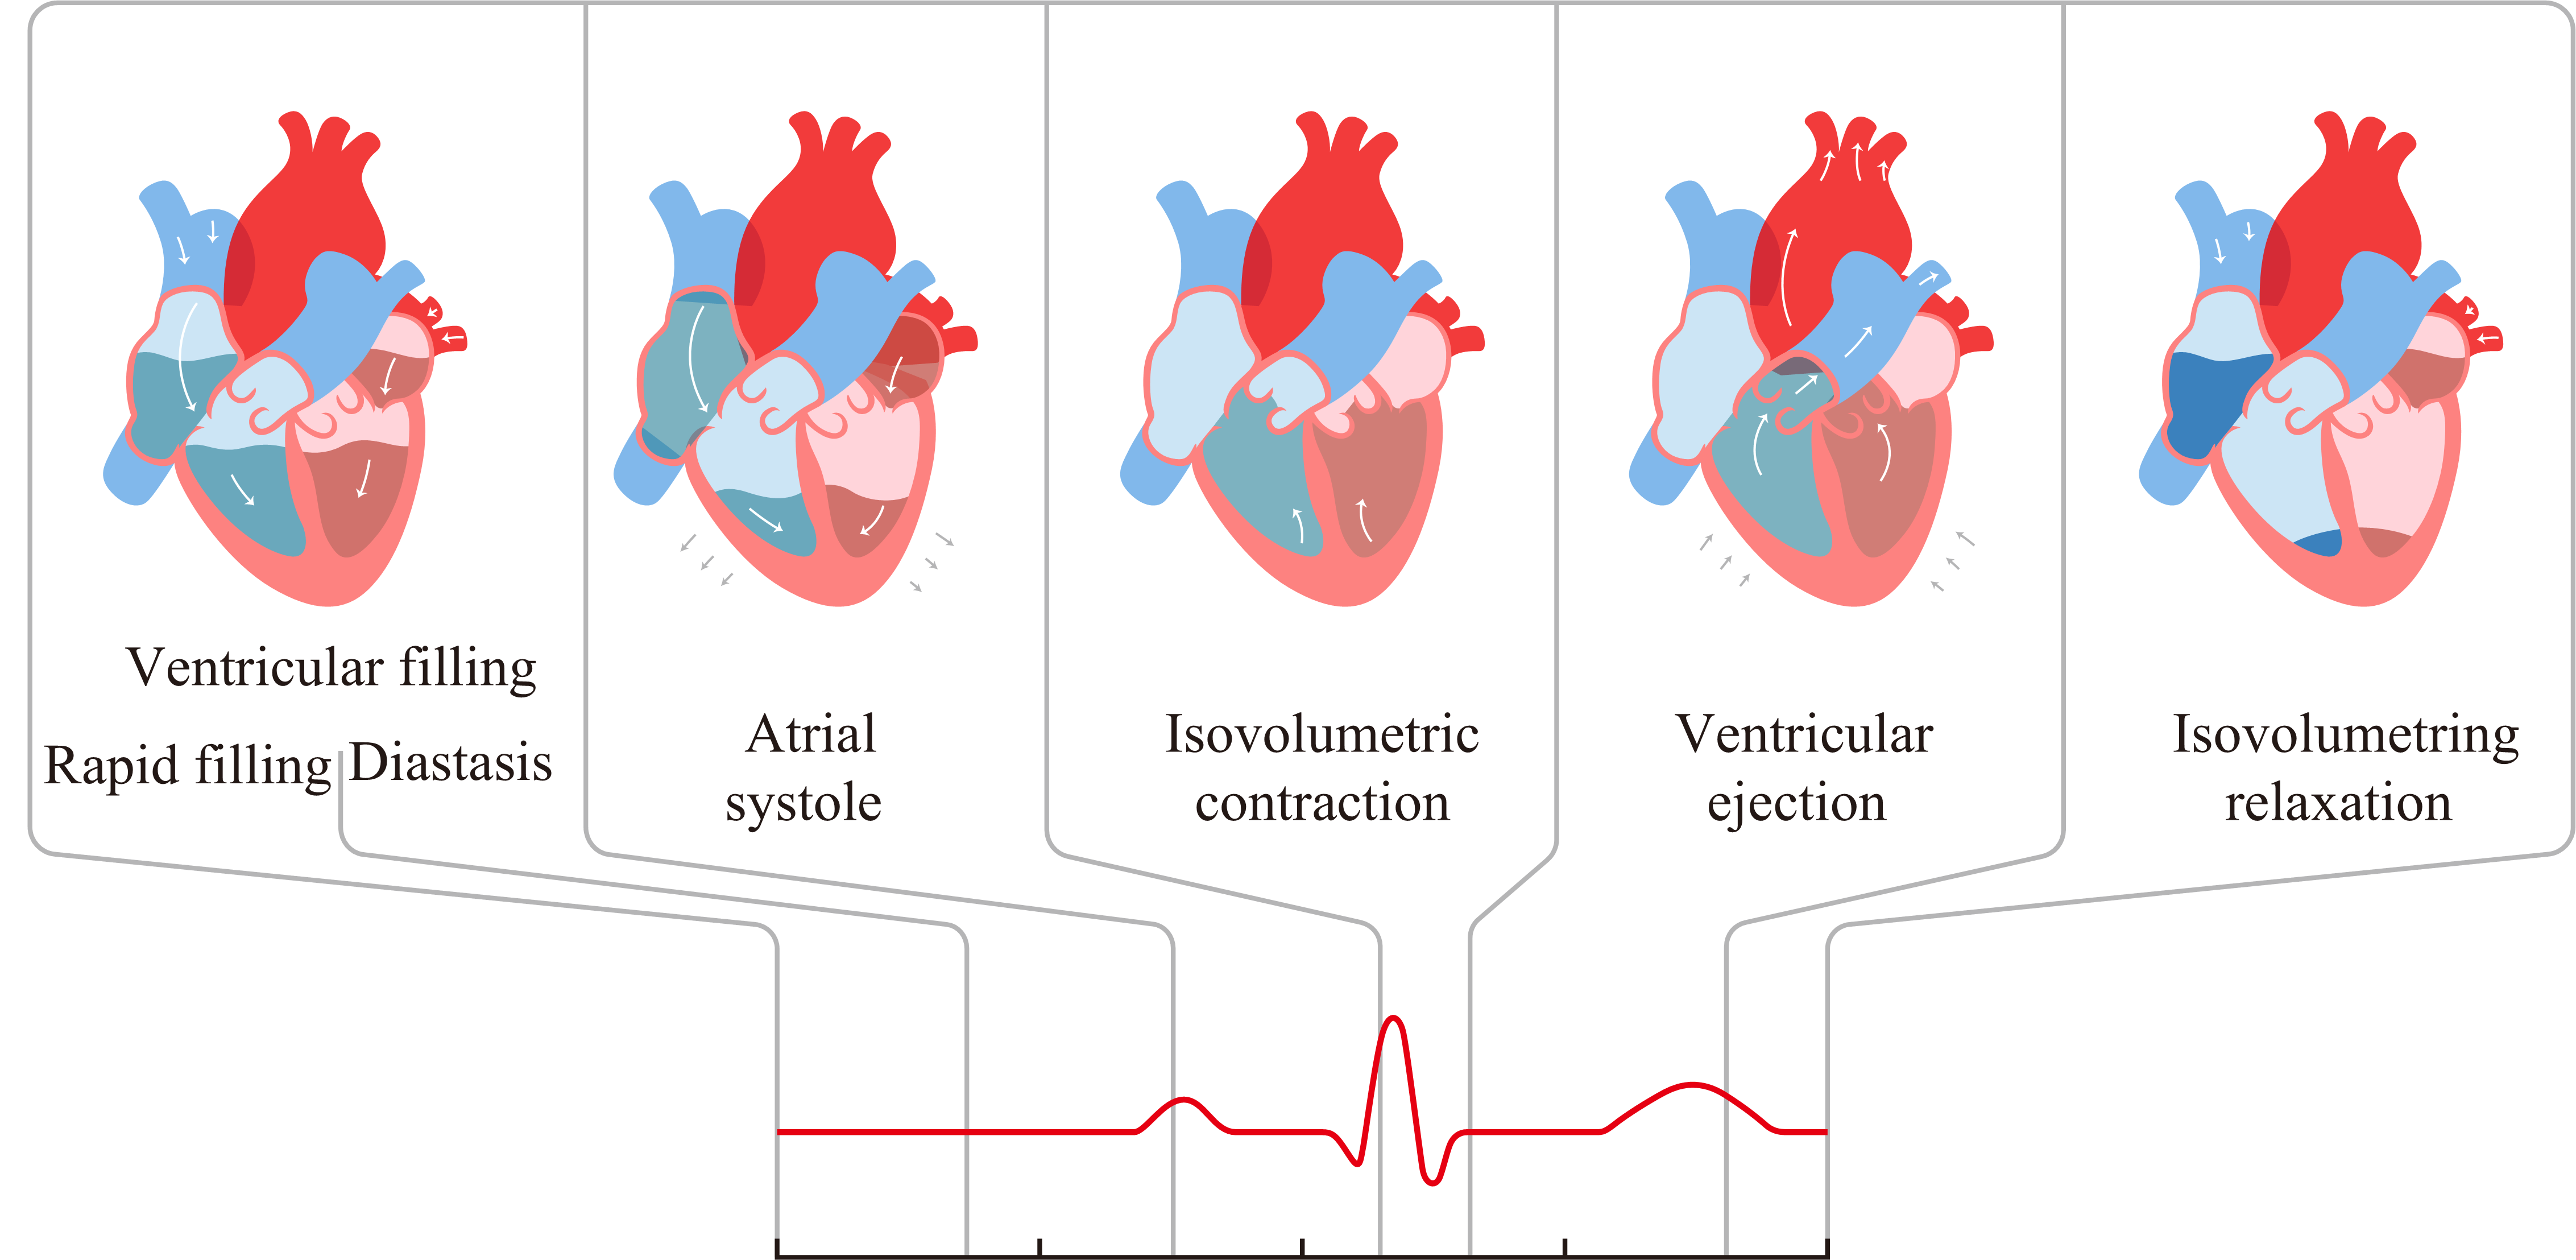
\includegraphics[width=8.5cm]{Figure/cycle}
    \caption{Illustration of the cardiac cycle, correlating the key electrical events of the ECG with their corresponding mechanical phases, such as atrial systole and ventricular ejection.}
    \label{fig:1}
\end{figure}


Among all implantable communication scenarios, the multi-chamber Leadless Pacemakers (LCPs) system represents the ultimate “proving ground” for the robustness of GCC technology~\cite{middour2021leadless, malaczynska2023leadless,li2025dynamic}. This is because the intracardiac environment imposes a uniquely challenging channel dynamic: the millimeter-scale electrodes of LCPs experience constant changes in relative geometry with every heartbeat, while the conductivity of the surrounding blood and myocardium fluctuates with the phases of contraction and blood flow, rendering the link gain markedly non-stationary. Consequently, understanding and modeling this complex Intracardiac Communication (CIC) channel has been a central focus of research. Early, foundational investigations logically began by establishing the baseline transmission properties through static or quasi-static models, employing finite element analysis, numerical simulations, and \textit{in-vivo} animal studies~\cite{bereuter2018fundamental, wang2024analysis,khaleghi2020conductive, maldari2020wide}. As the field matured, research has necessarily shifted to capture the channel's dynamic nature. For instance, the work of \cite{chen2022investigation} provided valuable experimental insights into these dynamics via an \textit{ex-vivo} platform, while our group's prior work established a time-varying equivalent circuit model for the channel under a normal cardiac cycle~\cite{wei2024time}.


These foundational studies are indispensable first steps. However, a critical challenge emerges as research transitions from theoretical feasibility to clinical robustness. Many existing CIC transceiver designs, in their early stages, inevitably rely on static or averaged channel models~\cite{ryser2022modulation,bereuter2019leadless,khaleghi2020conductive}. This idealized approximation, while convenient for initial analysis, masks a crucial fact: the intracardiac channel dynamics exist on two distinct levels.The first level is the ``healthy dynamic.'' As illustrated in Fig.~\ref{fig:1}, the regular heartbeat induces predictable, periodic fluctuations in channel gain. This baseline dynamic itself precludes the use of static receivers and establishes the fundamental necessity for employing automatic gain control (AGC). However, a second, more severe and clinically significant level is the ``pathological dynamic.'' A representative form of this condition, an Atrioventricular block(AVB) as shown in Fig.~\ref{fig:0}, is characterized by intermittent conduction failure that breaks the original predictable rhythm and introduces irregular, abrupt, and deeper channel fades.This latter condition exposes the inherent response latency bottleneck of conventional feedback-only AGCs, which rely purely on a ``post-event" reaction and thus struggle to maintain link reliability.


%这些基础性研究是不可或缺的第一步。然而，当研究从理论可行性向临床稳健性过渡时，一个关键挑战浮现出来。许多现有的心内通信（CIC） transceiver设计在其早期阶段，不可避免地依赖于静态或平均信道模型[参考文献{ryser2022modulation, bereuter2019leadless, khaleghi2020conductive}]。这种理想化的近似虽然便于初步分析，但掩盖了一个关键事实：心内信道动态存在于两个不同的层面。
%第一个层面是“健康动态”。如图\ref{fig:1}所示，正常的心跳会引起信道增益出现可预测的周期性波动。这种基线动态本身就排除了使用静态接收器的可能，并确立了采用自动增益控制（AGC）的基本必要性。
%然而，第二个层面是“病理性动态”，它更为严重且具有重要的临床意义。这种情况的一种典型表现是图\ref{fig:0}所示的房室（AV）传导阻滞，其特征是间歇性传导障碍，这会打破原本可预测的节律，并导致不规则、突然且更深的信道衰落。在这些情况下，传统的反馈控制机制纯粹依赖于“事后”反应，由于其固有的响应延迟，难以及时、稳定地维持链路可靠性，这对将原型转化为临床可靠的设备构成了根本性障碍。


The choice of receiver architecture is paramount in addressing this ultimate challenge. Given the stringent constraints on power and complexity in LCPs, the Super-Regenerative Receiver (SRR) architecture is a promising candidate due to its potential for high sensitivity at very low power~\cite{frey2013improved,macfarlane1948theory}. The SRR, however, is a double-edged sword: its performance exhibits extreme sensitivity to the input signal amplitude~\cite{chen2007fully,vidojkovic20112}. This sensitivity stems from its operating principle, where the envelope growth rate is directly seeded by the input signal. Consequently, a drop in channel gain translates into a lower effective signal-to-noise ratio (SNR) at the decision point, causing a surge in the bit error rate (BER). Therefore, stabilizing the SRR's input amplitude within a narrow target window becomes the primary control objective.
%
%接收机架构的选择在应对这一终极挑战时至关重要。考虑到低功耗通信设备（LCPs）在功率和复杂度方面的严格限制，超再生接收机（SRR）架构因其能在极低功率下实现高灵敏度而成为极具潜力的候选方案[frey2013improved, macfarlane1948theory]。然而，超再生接收机是一把双刃剑：其性能对输入信号幅度表现出极高的敏感性[chen2007fully, vidojkovic20112]。这种敏感性源于其工作原理，即包络增长率直接由输入信号决定。因此，信道增益的下降会导致判决点的有效信噪比（SNR）降低，进而导致误码率（BER）激增。所以，将超再生接收机的输入幅度稳定在一个狭窄的目标范围内成为主要的控制目标。


\begin{figure}[!t]
    \centering
    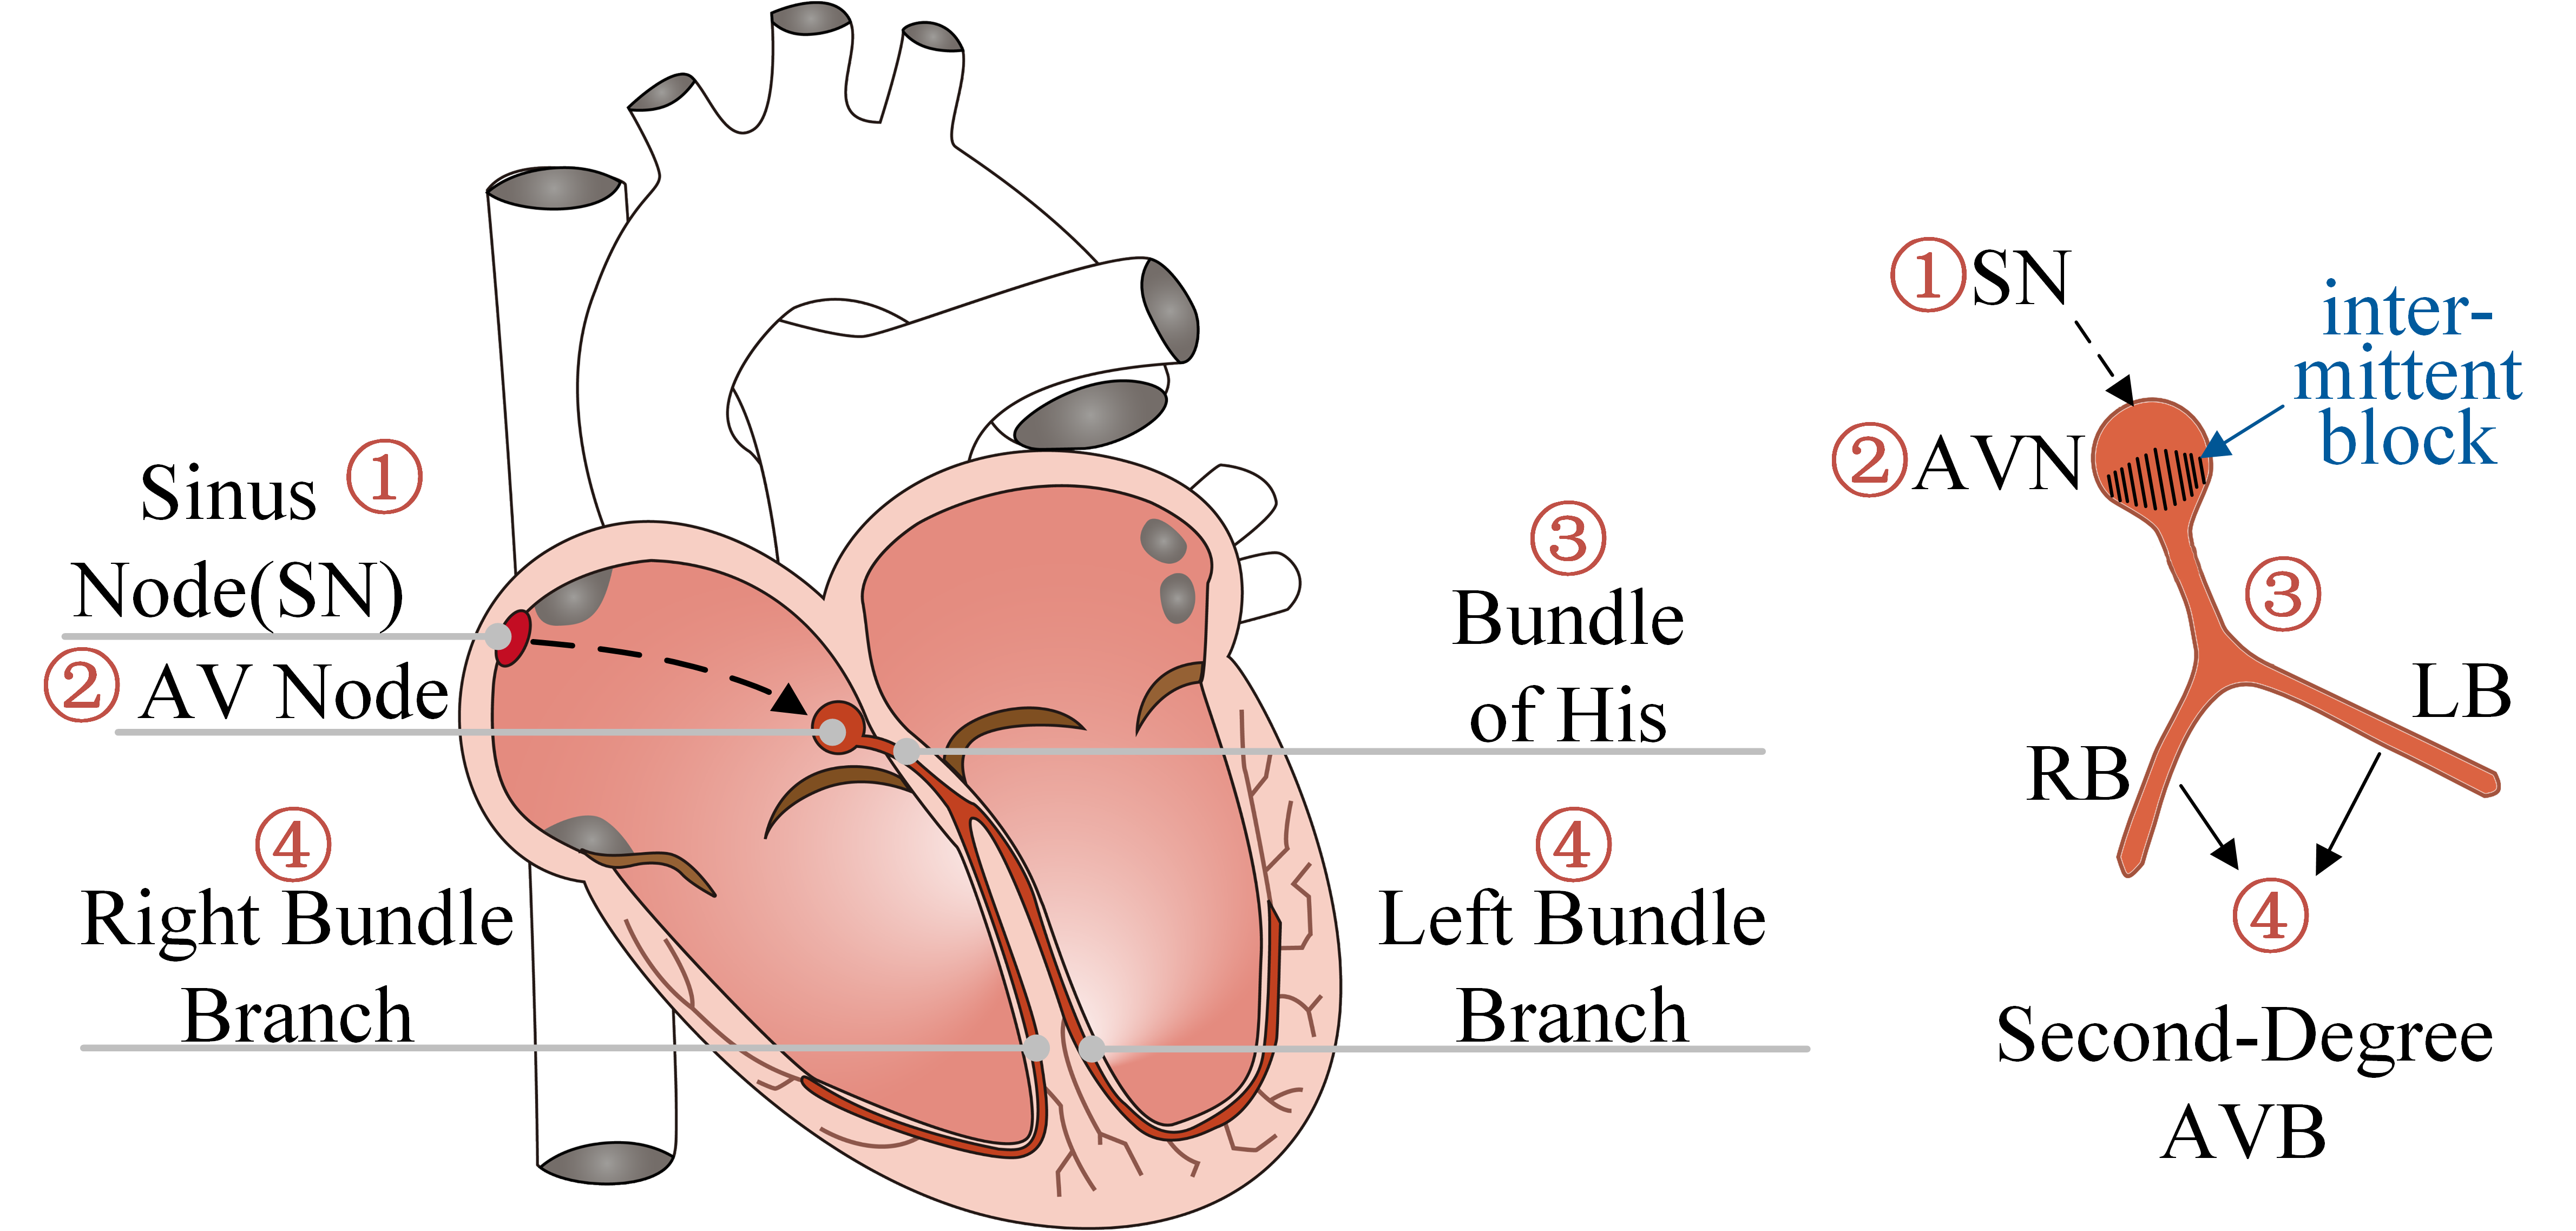
\includegraphics[width=8.3cm]{Figure/AVB}
    \caption{Schematic diagram of the cardiac conduction system and a representative Atrioventricular Block (Second-degree Type I).}
    \label{fig:0}
\end{figure}

AGC is thus an indispensable component. Yet, conventional AGC solutions often fail to achieve an optimal trade-off under LCP constraints. Fully analog AGCs, while fast, can suffer from poor linearity and imprecise control~\cite{Zhao2023AnAF}. Fully digital AGCs, while precise, incur computational overhead and power consumption incompatible with the microwatt-level budget of LCPs~\cite{Li2020DigitalAC}. Furthermore, a feedback-only loop is limited by its bandwidth and struggles to track large, step-like disturbances characteristic of cardiac beats. A more advanced strategy is needed, one that can proactively pre-compensate for these large, predictable disturbances.


In response to this imperative, this paper introduces a novel receiver front-end based on an SRR, deeply co-designed with a hybrid analog-digital AGC architecture. This architecture strategically combines the rapid response of an analog front-end with the fine-grained control of the digital domain to achieve robust compensation for dynamic CIC channel gain fluctuations. The main contributions of this work are as follows:


A beat-synchronous two-degree-of-freedom (2-DOF) active compensation strategy is proposed. It operates without an external electrocardiogram (ECG), using the peak RSSI of each beat as a proxy for the cardiac rhythm to combine predictive feedforward with incremental PID feedback, proactively stabilizing gain against aperiodic, pathologically-triggered step changes.


\begin{itemize}
    \item A beat-synchronous two-degree-of-freedom control (2-DOF) active compensation strategy is proposed, which operates without an external ECG. The peak RSSI of each beat is used as a proxy for the cardiac rhythm, combining predictive feedforward with incremental PID control to proactively stabilize the gain against aperiodic, pathologically-triggered step changes.

    \item A programmable ex-vivo platform was developed to emulate the pathological dynamics of Mobitz Type I AVB. This controllable and repeatable setup enables the systematic evaluation of the communication link under clinically relevant and reproducible adverse channel conditions.

    \item A dual-path quantitative evaluation framework was established. It integrates Hardware-in-the-Loop (HIL) for transient control characterization with ex-vivo experiments for end-to-end BER assessment, building and validating a clear causal link from control metrics to link reliability across multiple heart samples.
\end{itemize}



\section{Methods}
\label{sec:Methods}

\subsection{Challenges of the Dynamic Intracardiac Channel and Its Impact on SRR Performance}
\label{subsec:channel_and_impact}

The fundamental challenge for efficient communication between multi-chamber LCPs arises from the dynamic and complex physiological environment of the heart. The periodic electromechanical activity of the heart induces significant and time-varying fluctuations in the CIC channel gain, $G_c(t)$~\cite{wei2024time}. Under pathological conditions requiring pacing intervention, such as ``missed beats" caused by conduction block, the channel dynamics become even more complex and unpredictable than during a normal sinus rhythm. This study, therefore, aims to design an adaptive receiver capable of maintaining robust communication in such a harsh and non-stationary channel.

Given the ultra-low-power constraints of LCPs, the SRR is a favored architecture due to its high sensitivity and simple structure. However, the performance of an SRR is exceptionally sensitive to the input signal amplitude, $A_{in}(t)$. This characteristic stems from its operating principle: during the regeneration phase, the net conductance of the oscillator tank is negative ($G = G_o - G_N < 0$), causing the voltage envelope $V_{env}(t)$ to grow exponentially from an initial value set by the input signal $A_{in}(t)$:
\begin{equation}
    V_{env}(t) \approx A_{in}(t) \cdot \exp\left(\frac{|G|}{2C}t\right), \quad \text{for } t \in [0, T_{\text{regen}})
\end{equation}
where $T_{\text{regen}}$ is the regeneration period. Consequently, within a fixed quench period, the final detected envelope amplitude is a monotonically increasing function of $A_{in}(t)$. In a front-end without adaptive control, the SRR's input amplitude $A_{in}(t)$ is directly coupled with the time-varying channel:
\begin{equation}
    A_{in}(t) = A_{tx} \cdot G_{LNA} \cdot G_c(t)
\end{equation}
where $A_{tx}$ and $G_{LNA}$ are the transmitted signal amplitude and the low-noise amplifier (LNA) gain, respectively. Fluctuations in channel gain $G_c(t)$ directly translate into variations in $A_{in}(t)$, which in turn cause drastic changes in the effective signal-to-noise ratio ($SNR_{eff}$) at the SRR's decision point. This relationship can be modeled as a monotonic function:
\begin{equation}
    P_e(t) = f_{\text{BER}}(SNR_{eff}(t)),  SNR_{eff}(t) \propto A_{in}^2(t)
\end{equation}
where $f_{\text{BER}}(\cdot)$ is a monotonically decreasing function. During deep channel fades, a sharp drop in $SNR_{eff}(t)$ causes the bit error rate $P_e(t)$ to approach 0.5, leading to instantaneous link failure. Therefore, stabilizing $A_{in}(t)$ is a prerequisite for reliable communication. Notably, the control scheme proposed herein does not rely on an external ECG signal; when the ECG is unavailable, the system can autonomously extract rhythmic information from the envelope of the received signal strength indicator (RSSI).

\subsection{Adaptive Receiver Architecture with Hybrid Gain Control}
\label{subsec:adaptive_architecture}

To address the aforementioned challenges, we propose an adaptive receiver architecture centered around a hybrid analog-digital automatic gain control (Hybrid-AGC) loop, as illustrated in Fig.~\ref{fig:framework}. The core objective of this architecture is to dynamically adjust the total front-end gain to precisely compensate for fluctuations in the channel gain $G_c(t)$, thereby providing a constant-amplitude input signal to the subsequent SRR core.


\begin{figure}[!t]
    \centering
    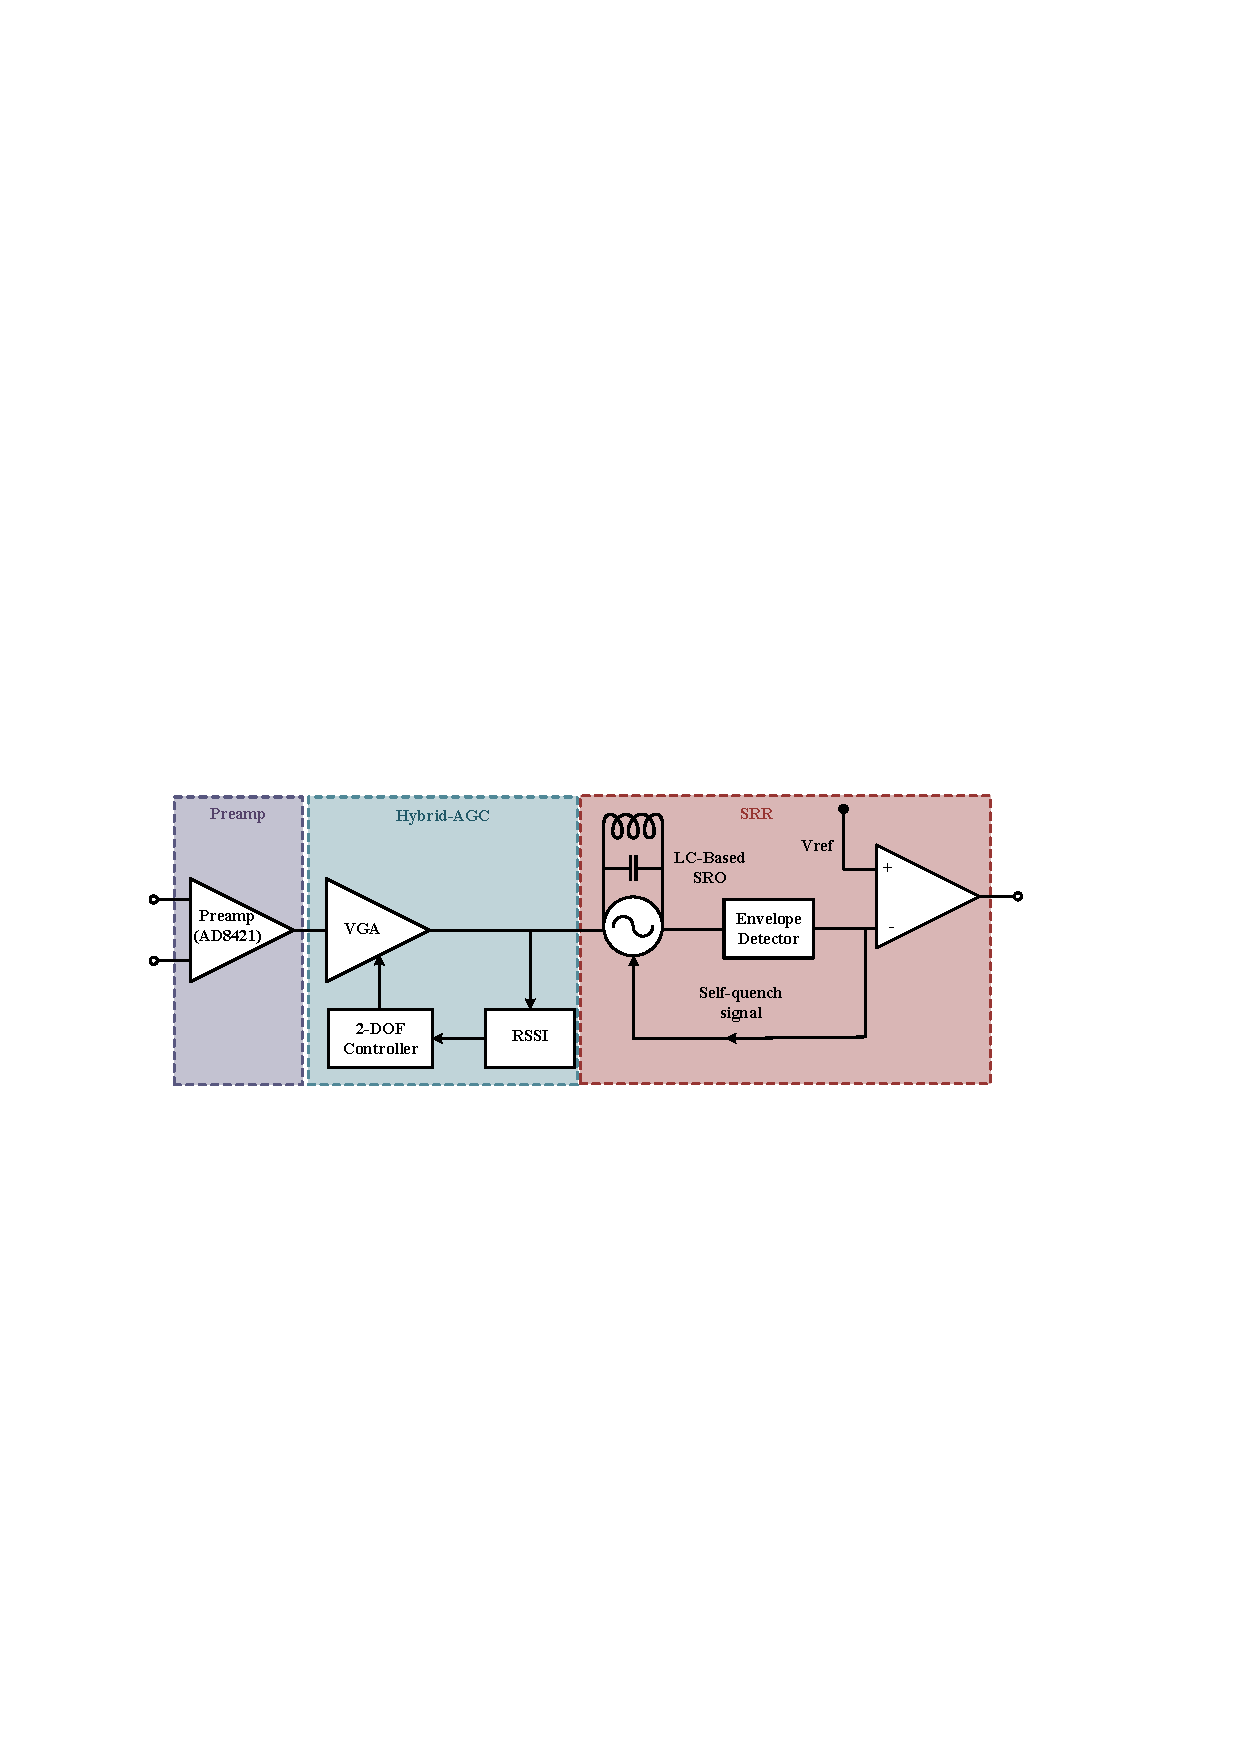
\includegraphics[width=8.3cm]{Figure/framework}
    \caption{Block diagram of the proposed adaptive receiver architecture. The core Hybrid-AGC module forms a closed loop, using a RSSI and a 2-DOF controller to dynamically adjust the VGA, thereby delivering a stabilized signal to the SRR stage.}
    \label{fig:framework}
\end{figure}


As depicted in the diagram, the receiver chain is divided into three functional stages. The signal first enters a fixed pre-amplification stage (Preamp), followed by the Hybrid-AGC module, which acts as the core regulation unit. This module forms a sophisticated negative feedback loop: a variable gain amplifier (VGA) amplifies the signal, and its output is simultaneously routed to the final SRR detection stage and monitored in real-time by a RSSI. The RSSI converts the signal envelope's strength into a corresponding DC voltage, which is then sampled by an analog-to-digital converter and fed to a digital 2-DOF controller. This controller compares the sampled value against a preset target, computes the error, and generates an updated gain control signal based on its control algorithm. This digital signal is converted back to an analog voltage by a digital-to-analog converter to precisely regulate the VGA's gain. This completes the closed-loop regulation, ensuring that the signal strength delivered to the SRR remains stable regardless of input channel variations.


\begin{algorithm}[t]
\caption{Beat-Synchronous 2-DOF Gain Stabilization with RSSI Prediction}
\label{alg:pid_control}
\begin{algorithmic}[1]
\setlength{\baselineskip}{1.2\baselineskip}  % 增加行距
\small  % 使用小号字体以适应单栏
\Require Target level $x^\star_{\text{dig}}$, $K_f$, $\alpha$, PID gains $(K_p,K_i,K_d,K_{aw})$, bounds $u_{\min},u_{\max}$, slew limit $\Delta u_{\max}$
\Ensure $V_c[k]$
\State Initialize: $I_{\text{prev}}\gets 0$, $D_{\text{prev}}\gets 0$, $e_{\text{prev}}\gets 0$
\State $\hat x_{\text{prev}}\gets x^\star_{\text{dig}}$, $u_{\text{final\_prev}}\gets 0$, $u_{\text{PID\_prev}}\gets 0$, $u_{\text{ff}}\gets 0$
\While{system running}
  \State $x[k]\gets$ Sample\_and\_digitize\_RSSI\_dB
  \If{new heartbeat detected}
    \State $x_{p}\gets$ Peak\_RSSI\_of\_previous\_beat\_dB
    \State $\hat x \gets (1-\alpha)\hat x_{\text{prev}}+\alpha x_{p}$
    \State $u_{\text{ff}}\gets K_f(x^\star_{\text{dig}}-\hat x)$
    \State $\hat x_{\text{prev}}\gets \hat x$
  \EndIf
  \State $e[k]\gets x^\star_{\text{dig}}-x[k]$
  \State $D[k]\gets \frac{T_d}{T_d+NT_s}D_{\text{prev}}+\frac{K_dN}{T_d+NT_s}(e[k]-e_{\text{prev}})$
  \Statex \hfill $\triangleright$ filtered derivative
  \State $u_{\text{PID}}[k]\gets u_{\text{PID\_prev}}+K_p(e[k]-e_{\text{prev}})$
  \Statex \hspace{3.5em} ${}+K_iT_se[k]+(D[k]-D_{\text{prev}})$
  \Statex \hfill $\triangleright$ incremental PID
  \State $u_{\text{tot}}[k]\gets u_{\text{ff}}+u_{\text{PID}}[k]$
  \State $u_{\text{final}}[k]\gets \text{clip}(u_{\text{tot}}[k], u_{\text{final\_prev}}\pm\Delta u_{\max})$
  \State \hfill $\triangleright$ slew limit
  \State $u_{\text{sat}}[k]\gets \text{clip}(u_{\text{final}}[k], u_{\min}, u_{\max})$
  \State \hfill $\triangleright$ saturation
  \State $V_c[k]\gets \text{DAC}(u_{\text{sat}}[k])$
  \State \textit{Update history for next iteration:}
  \State $D_{\text{prev}}\gets D[k]$, $e_{\text{prev}}\gets e[k]$
  \State $u_{\text{PID\_prev}}\gets u_{\text{PID}}[k]$, $u_{\text{final\_prev}}\gets u_{\text{final}}[k]$
\EndWhile
\end{algorithmic}
\end{algorithm}






\subsection{Loop Modeling, Stability, and Implementation}
\label{subsec:loop_modeling_and_stability}

To ensure the closed-loop system exhibits robust and predictable dynamic performance, we first establish a control-theoretic model for the AGC–SRR system, which guides the controller's design and tuning. We approximate the entire path from the VGA gain control input to the ADC output in the logarithmic domain as a first-order continuous-time system with a pure delay $\tau_d$: $\dot{x}(t) = -(1/\tau)x(t) + \gamma_c u(t-\tau_d)$. Discretization using a zero-order hold yields its discrete-time equivalent model:
\begin{equation}
    x[k+1] = \phi x[k] + \gamma u[k-d] + w[k]
\end{equation}
where $x[k]$ is the sampled RSSI value, $u[k]$ is the VGA gain control signal, and the mapping from continuous to discrete parameters is:
\begin{equation}
    \phi = e^{-T_s/\tau}, \quad \gamma = \gamma_c \tau (1 - e^{-T_s/\tau}), \quad d = \lceil \tau_d / T_s \rceil
\end{equation}

The term $w[k]$ represents model uncertainty and noise. The transfer function of the plant, $P(z)$, is therefore:
\begin{equation}
    P(z) = \frac{X(z)}{U(z)} = \frac{\gamma z^{-d}}{1 - \phi z^{-1}}
\end{equation}

The system's open-loop transfer function is $L(z)=C(z)P(z)$. Our design objective is to maintain closed-loop stability under all operating conditions, with a specific target of a phase margin $\ge 45^{\circ}$. This provides a clear optimization goal for tuning the PID parameters ($K_p, K_i, K_d$). The approximate relationship between the settling time $t_{\text{settle}}$ and the controller parameters further reveals their impact on dynamic performance:
\begin{equation}
t_{\mathrm{settle}}\approx \frac{4}{\zeta\omega_n}, \quad \text{where} \quad
\omega_n \propto \sqrt{K_p}, \; \zeta \propto K_d
\end{equation}

To translate this theoretical model into a high-performance practical controller, we integrated several key implementation techniques. To suppress the amplification of high-frequency noise by the derivative term, we employed a first-order low-pass filter to smooth the rate of error change, with its update rule given below (recommended parameters: $T_d=2T_s$, $N=10$):
\begin{equation}
    D[k]=\frac{T_d}{T_d+N T_s}D[k-1]+\frac{K_d N}{T_d+N T_s}(e[k]-e[k-1])
\end{equation}

Simultaneously, to prevent integral windup when the VGA gain saturates, we implemented an anti-windup mechanism via back-calculation, where the integral accumulator is corrected based on the saturation error:
\begin{equation}
    I[k+1]=I[k]+K_i T_s e[k]+K_{aw}(u_{\text{sat}}[k]-u[k])
\end{equation}
where $u_{\text{sat}}[k]$ is the saturated control output. Furthermore, during the preamble of a data packet, we temporarily freeze the integral and derivative channels, relying solely on proportional control for rapid coarse adjustment to avoid overshoot from the initial step response.

\subsection{Beat-Synchronous 2-DOF Control Algorithm with RSSI Prediction}
\label{subsec:2dof_control_algorithm}

Despite these optimizations, a conventional feedback-only PID controller is still limited by its loop bandwidth in terms of response speed and overshoot when facing the abrupt, step-like changes in channel gain inherent to the cardiac cycle. While a well-tuned PID can manage the rhythmic, predictable steps of a healthy heart to some degree, its purely reactive nature proves critically insufficient for the chaotic dynamics of pathological conditions. The core challenge shifts from managing periodicity to compensating for unpredictability during events like the ``missed beats" in an Atrioventricular block. To overcome this bottleneck of unpredictability, we propose a 2-DOF control strategy that combines beat-synchronous feedforward control with PID feedback.

The fundamental principle of this strategy is rooted in the direct mapping between cardiac mechanics and received signal strength. As established in prior work~\cite{li2025Adynamic,li2025dynamic}, the heart's mechanical pumping action, characterized by the cyclical filling and ejection of blood—causes significant changes in both the geometry between the electrodes and the electrical properties of the transmission medium. These hemodynamic shifts directly modulate the channel gain ($G_c(t)$). The RSSI provides a real-time measurement of this gain, effectively serving as an electrical proxy for the heart's mechanical rhythm. It is this robust link that allows our system to leverage the heart's rhythmicity. By analyzing the RSSI envelope, the controller can autonomously identify beat boundaries and characterize each beat's channel quality by its peak RSSI value forming the basis for prediction.


Based on this, we employ a computationally lightweight Exponential Moving Average (EMA) model to predict the peak RSSI of the next beat:
\begin{equation}
\hat{x}_{k+1} = (1-\alpha)\hat{x}_k + \alpha x_k, \quad \alpha \in [0.2, 0.3]
\end{equation}
where $\hat{x}_{k+1}$ is the prediction for the next beat's peak RSSI. Our 2-DOF controller combines predictive compensation for the slowly varying component of the channel (beat-level jumps) with feedback regulation for fast-varying residuals. Ideally, the required VGA gain compensation (in dB) is $g_{vga}^*(t) = x^* - (g_c(t) + g_{lna} + g_{tx})$. Upon detecting the start of a new beat, the controller first calculates a feedforward control signal, $u_{\mathrm{ff}}$:
\begin{equation}
    u_{\mathrm{ff}}[k+1] = K_f (x^* - \hat{x}_{k+1}), \quad u_{\mathrm{ff}} \in [-8, 8] \text{ dB}
\end{equation}

This feedforward term is added to the incrementally implemented PID feedback output, $u_{\mathrm{PID}}$, to form the total control signal:
\begin{equation}
\begin{aligned}
    u_{\mathrm{PID}}[k] =\ & u_{\mathrm{PID}}[k-1] + K_p(e[k]-e[k-1]) \\
    & + K_i T_s e[k] + (D[k]-D[k-1])
\end{aligned}
\end{equation}
\begin{equation}
u_{\mathrm{total}}[k] = u_{\mathrm{ff}}[k] + u_{\mathrm{PID}}[k]
\end{equation}

To prevent rapid changes from stressing the hardware, we also apply a slew-rate limiter to the total control output:
\begin{equation}
    \begin{aligned}
    u_{\text{final}}[k] =\ & \text{clip}(u_{\text{total}}[k], u_{\text{final}}[k-1]\\
    &  - \Delta u_{\text{max}}, u_{\text{final}}[k-1] + \Delta u_{\text{max}})
     \end{aligned}
\end{equation}

Furthermore, to enhance robustness, the system includes a de-rating strategy: if the prediction error remains below a threshold for several consecutive beats, the feedforward gain $K_f$ is temporarily zeroed, and the system reverts to a pure PID mode until the next large jump is detected. The complete control logic, which integrates prediction, feedforward, feedback, and multiple robustness enhancements, is formalized in Algorithm~\ref{alg:pid_control}.




\section{Experimental Methodology and Setup}
\label{sec:methodology}

\begin{figure}[!t]
    \centering
    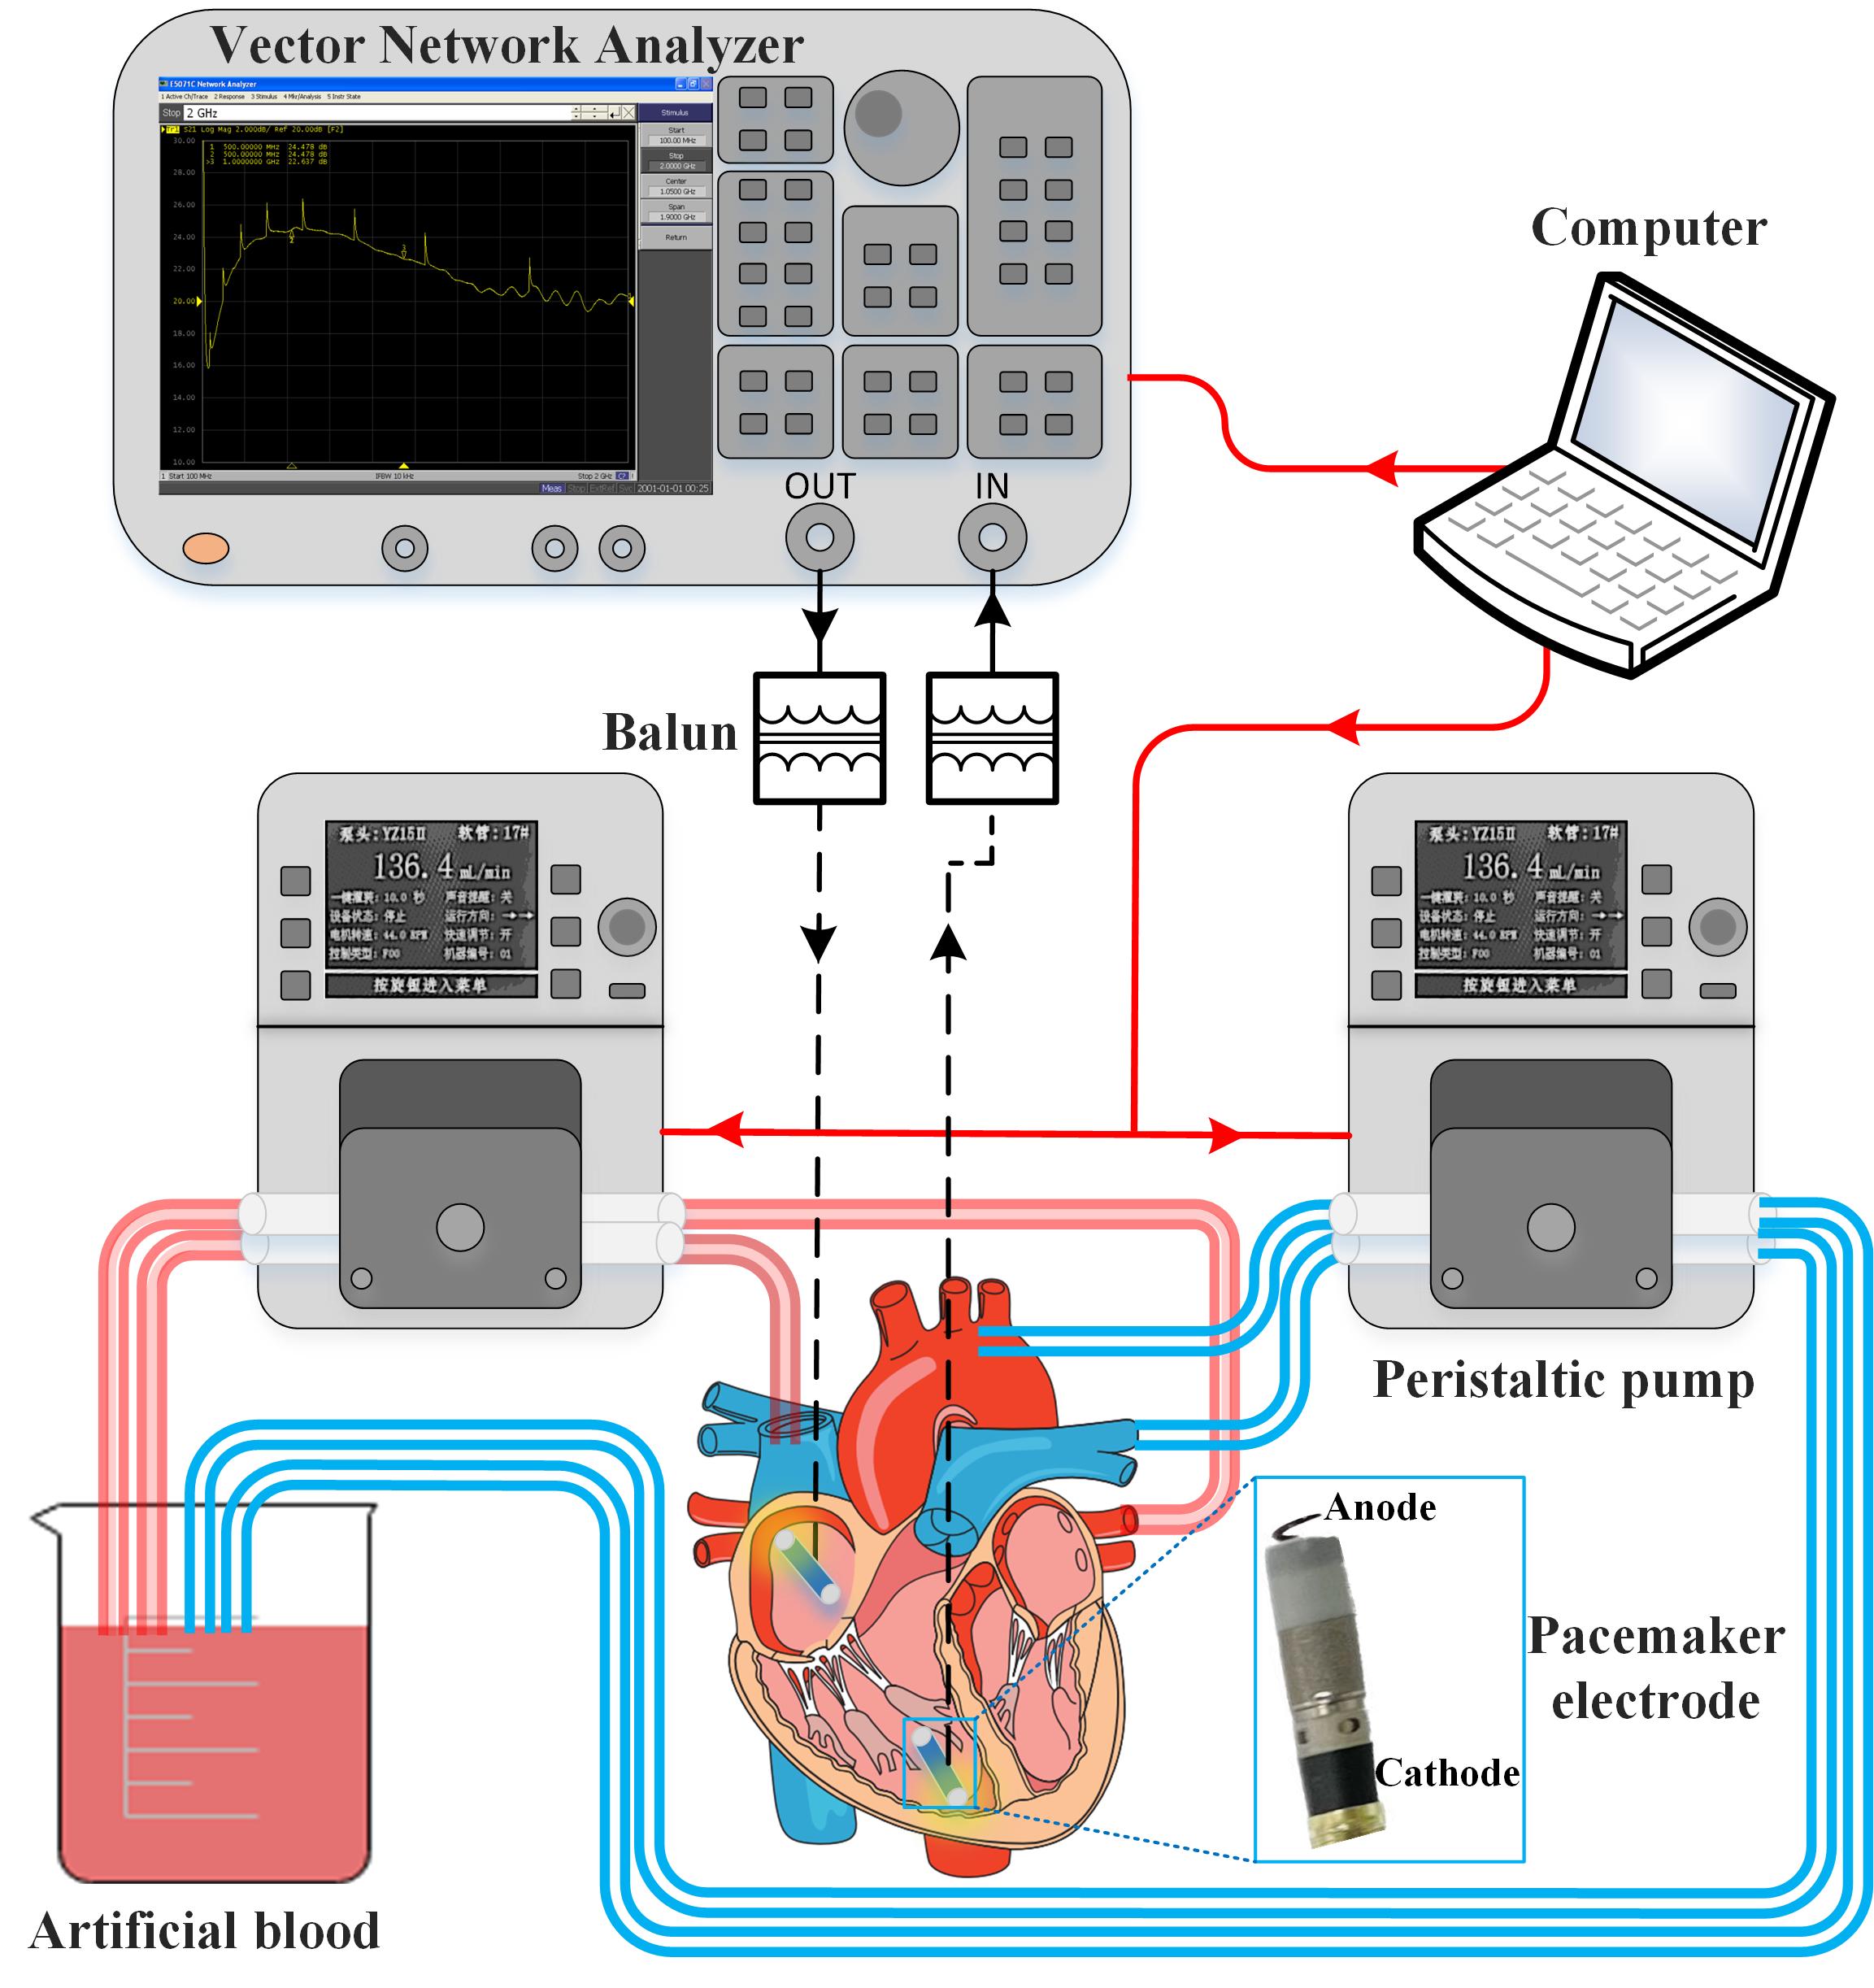
\includegraphics[width=0.9\columnwidth]{Figure/measure_setup}
    \caption{Photograph of the assembled experimental testbed, showing the peristaltic pump system, the cannulated isolated porcine heart, signal generation instruments, and the custom-developed receiver module. A 1:1 balun is used for current isolation.}
    \label{fig:agc_test_schematic}
\end{figure}


\begin{table}[!t]
\centering
\caption{Cardiac Cycle Phases and Corresponding Chamber Volumes}
\begin{tabular}{cccc}
\hline
\textbf{Phase} & \textbf{Duration (s)} & \textbf{\begin{tabular}[c]{@{}c@{}}Left Volume\\ (mL)\end{tabular}} & \textbf{\begin{tabular}[c]{@{}c@{}}Right Volume\\ (mL)\end{tabular}} \\ \hline
Isovolumic Relaxation & 0.07 & 120.00 & 150.00 \\
Rapid Filling & 0.11 & 173.44 & 202.88 \\
Diastasis & 0.22 & 191.25 & 220.50 \\
Atrial Systole & 0.10 & 215.00 & 244.00 \\
Isovolumic Contraction & 0.05 & 215.00 & 244.00 \\
Rapid Ejection & 0.10 & 151.67 & 181.34 \\
Reduced Ejection & 0.15 & 120.00 & 150.00 \\ \hline
\end{tabular}
\label{tab:volume_data}
\end{table}

To rigorously validate the proposed adaptive receiver architecture and its core 2-DOF control strategy, we established a high-fidelity ex-vivo experimental methodology. The cornerstone of this methodology is an isolated heart perfusion platform in Fig.~\ref{fig:agc_test_schematic}, which utilizes a freshly excised porcine heart as its biological core to maximally replicate the authentic intracardiac communication environment. A dual-channel peristaltic pump system circulates a specially formulated blood-mimicking fluid, matched to the conductivity of human blood at 37°C~\cite{maldari2020wide, gabriel1996dielectric
}. This setup, governed by a host computer executing precise temporal control over chamber volumes, achieves a high-fidelity simulation of intracardiac hemodynamics.

We contend that a truly robust adaptive system must maintain performance under harsh channel conditions characterized by both gradual and abrupt variations.
Consequently, we deliberately selected and implemented Mobitz Type I AVB as a representative pathological channel model.
The key advantage of this model is its inherent Wenckebach phenomenon, where channel parameters progressively deteriorate before a ``dropped beat,\("\) and the dropped beat itself manifests as an abrupt step-change in channel gain.
Our platform was programmed to precisely replicate the hemodynamic signatures of this AVB model, based on published human cardiac volume data~\cite{maceira2010reference, 2006Normalized, 2006Reference, 2013Reference, chen2022investigation}, with the specific parameters for each phase of the cardiac cycle detailwith the specific parameters for each phase of the cardiac cycle detailed in Table~\ref{tab:volume_data}.
The dynamic mappings for both normal sinus rhythm (NSR) and our AVB model are illustrated in Fig.~\ref{fig:nsr_mapping} and Fig.~\ref{fig:avb_mapping}, respectively.


Upon this high-fidelity platform, we instituted a direct comparative evaluation framework. This framework benchmarks our proposed 2-DOF controller, which integrates beat-synchronous predictive feedforward, against a well-tuned conventional feedback-only PID controller (serving as the baseline) and an open-loop configuration with no AGC. System performance was quantified using a suite of key metrics covering both transient dynamics and steady-state communication quality. The former includes settling time ($t_{\text{settle}}$) and maximum overshoot, while the latter is assessed by the end-to-end Bit Error Rate (BER). Across all experiments, the physical link setup remained constant: a \SI{1}{\mega\hertz} OOK signal with an average power of \SI{-10}{dBm} was generated and coupled to the right atrium, while our custom-developed SRR receiver, integrating the different control strategies, was connected to an electrode in the right ventricle.

Our evaluation strategy was strategically bifurcated into two complementary phases. First, to precisely assess the intrinsic transient response capabilities of the controller, independent of the complexities of the biological specimen, we employed a HIL simulation strategy. In this setup, the controller hardware under test (MCU) and its actuator (VGA) were physical devices, but their RF environment was digitally simulated in real-time by a host computer. The computer calculated the requisite signal strength at the SRR input based on predefined channel gain step sequences (5 dB, 10 dB, 15 dB) and the MCU's real-time output, then converted this value into an analog RSSI signal via a high-speed DAC to close the loop. Analyzing the controller's response to these step disturbances allowed for precise quantification of its settling time and maximum overshoot.

Second, communication reliability, the ultimate measure of the system's practical utility, was evaluated under the continuously dynamic pathological channel conditions generated by the isolated heart platform. As depicted in Fig.~\ref{BER}, a complete transceiver and analysis chain was established to conduct long-duration transmissions of a pseudo-random binary sequence (PRBS) for the no-AGC, PID, and 2-DOF configurations under the simulated AVB rhythm, enabling the calculation of BER at various data rates. To ensure the scientific rigor and reproducibility of all findings, the entire set of experiments was repeated in three independent porcine heart preparations (N=3), with five technical replicates for each measurement (n=5).




\begin{figure}[!t]
    \centering
    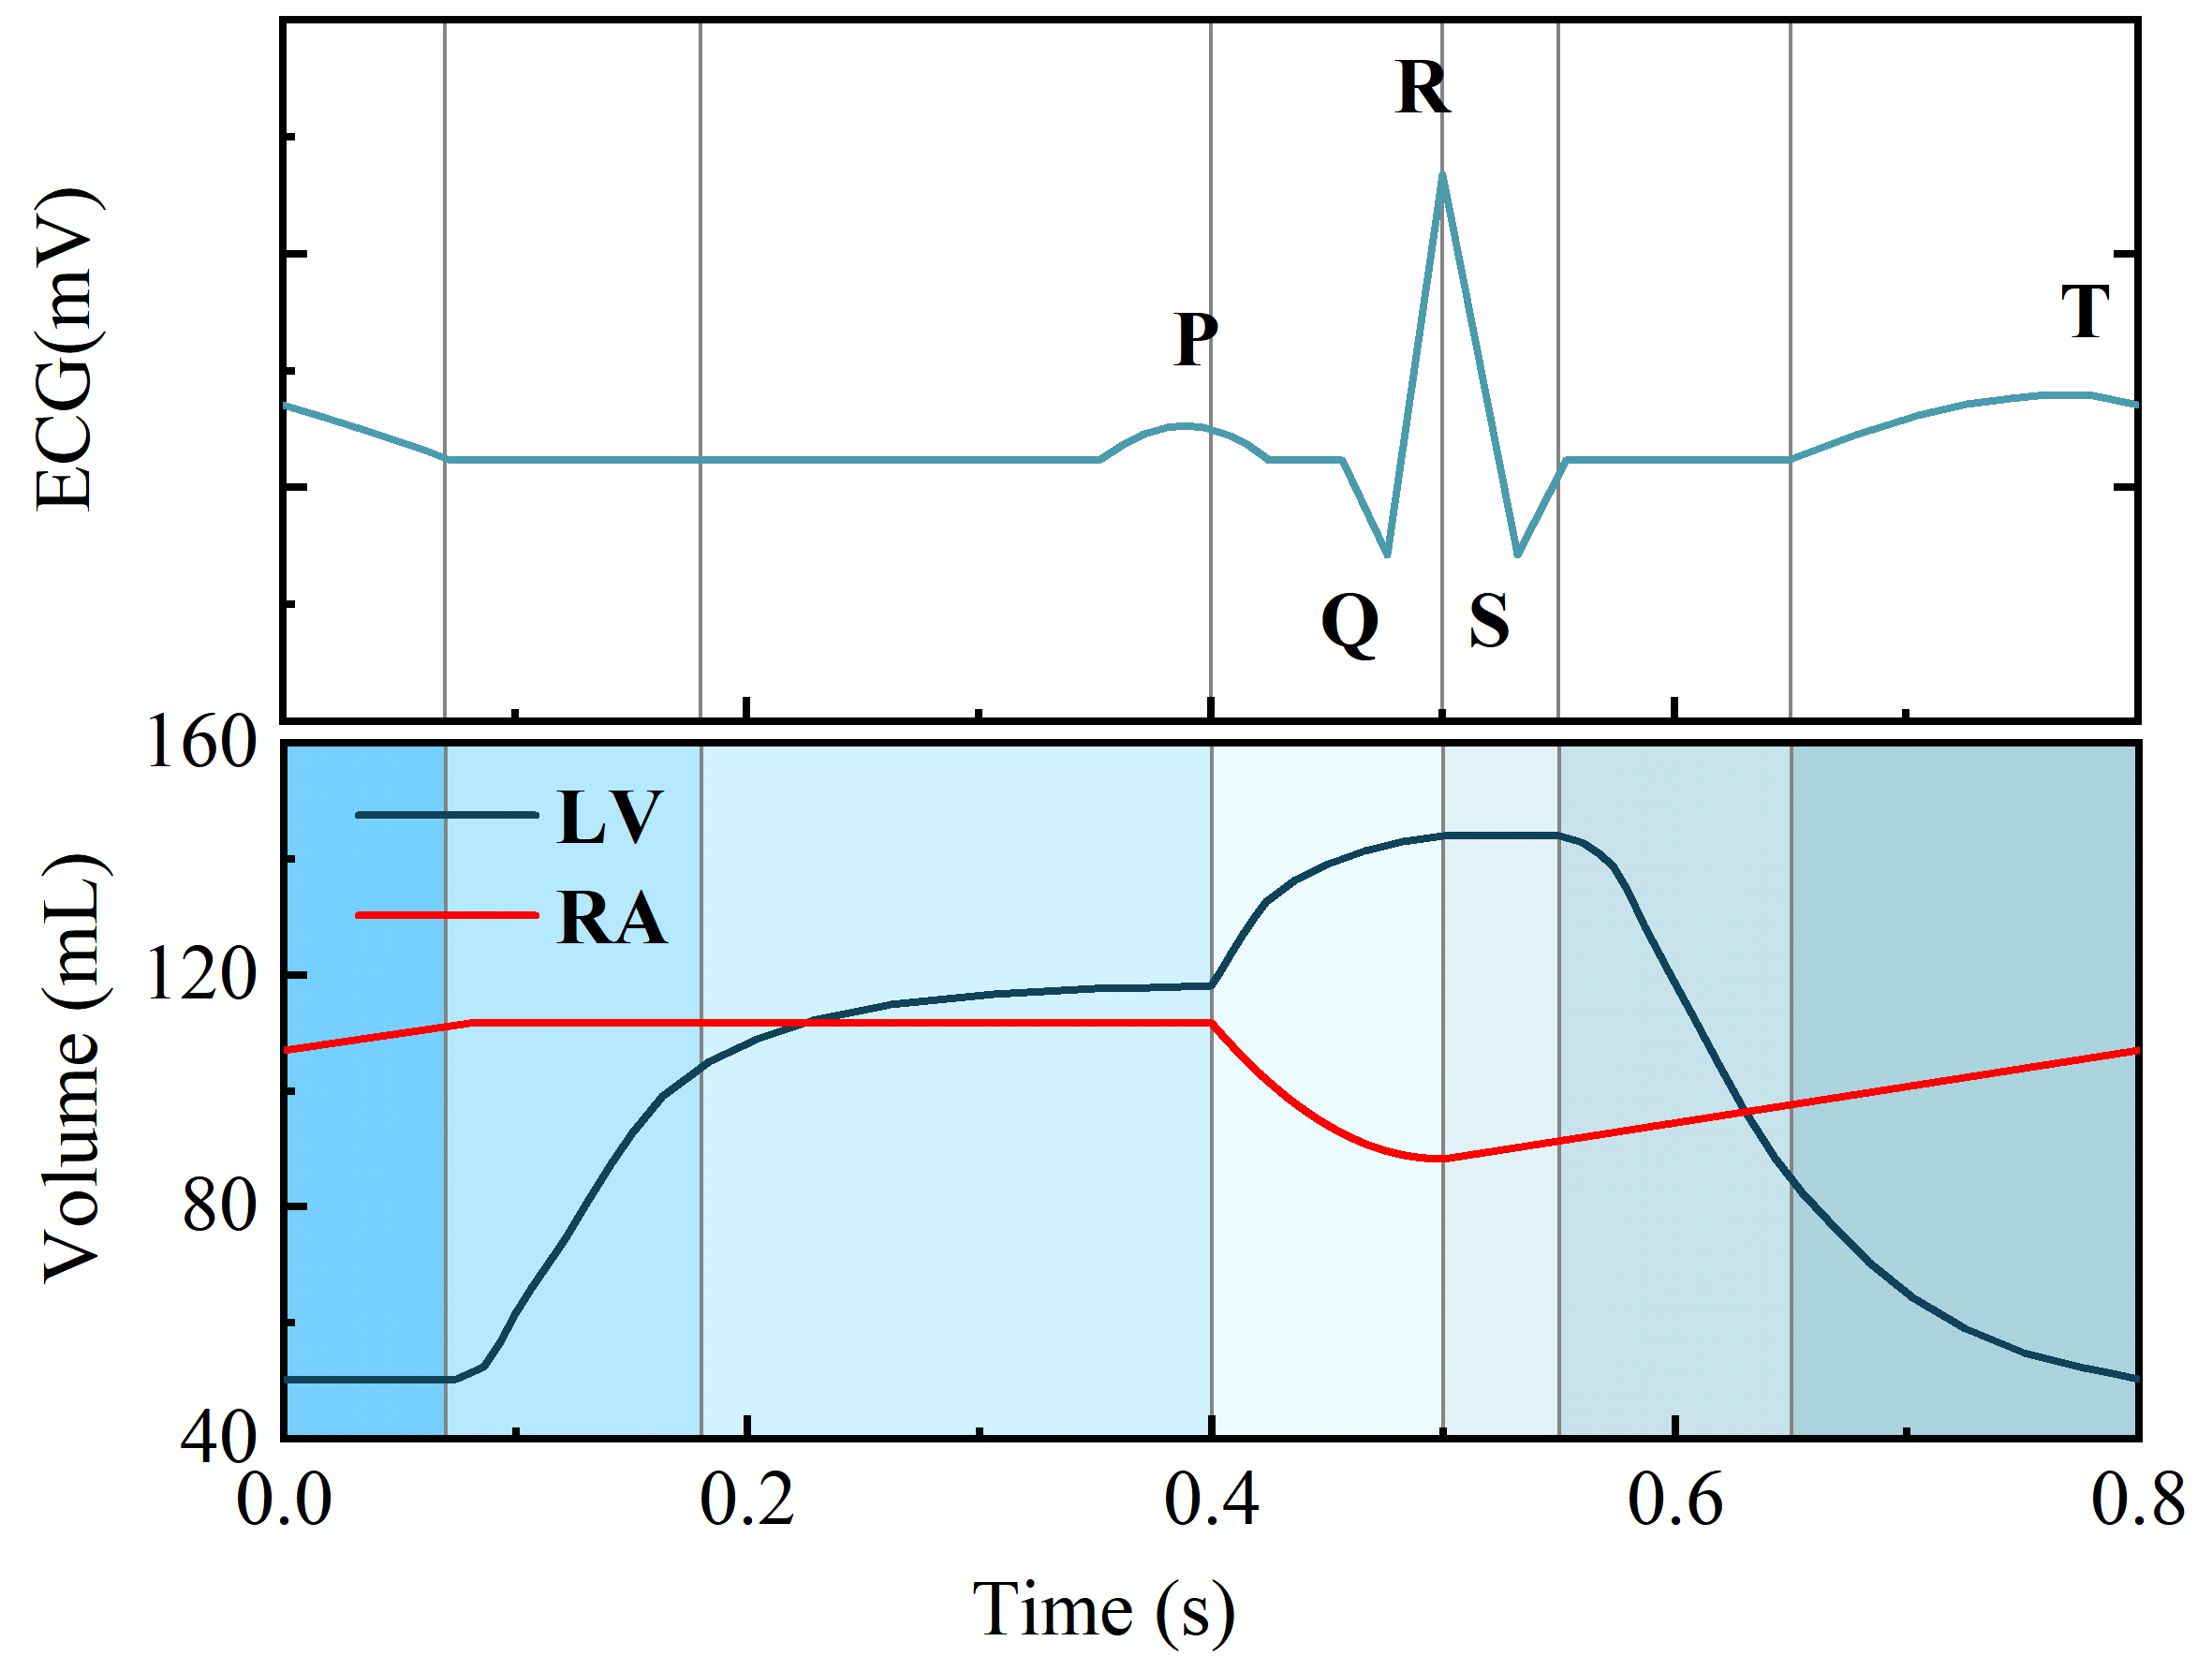
\includegraphics[width=0.9\columnwidth]{Figure/Nor_Vol}
    \caption{Dynamic mapping between ECG and right-sided chamber volume for the simulated NSR, serving as the baseline model for a healthy heart.}
    \label{fig:nsr_mapping}
\end{figure}

\begin{figure}[!t]
    \centering
    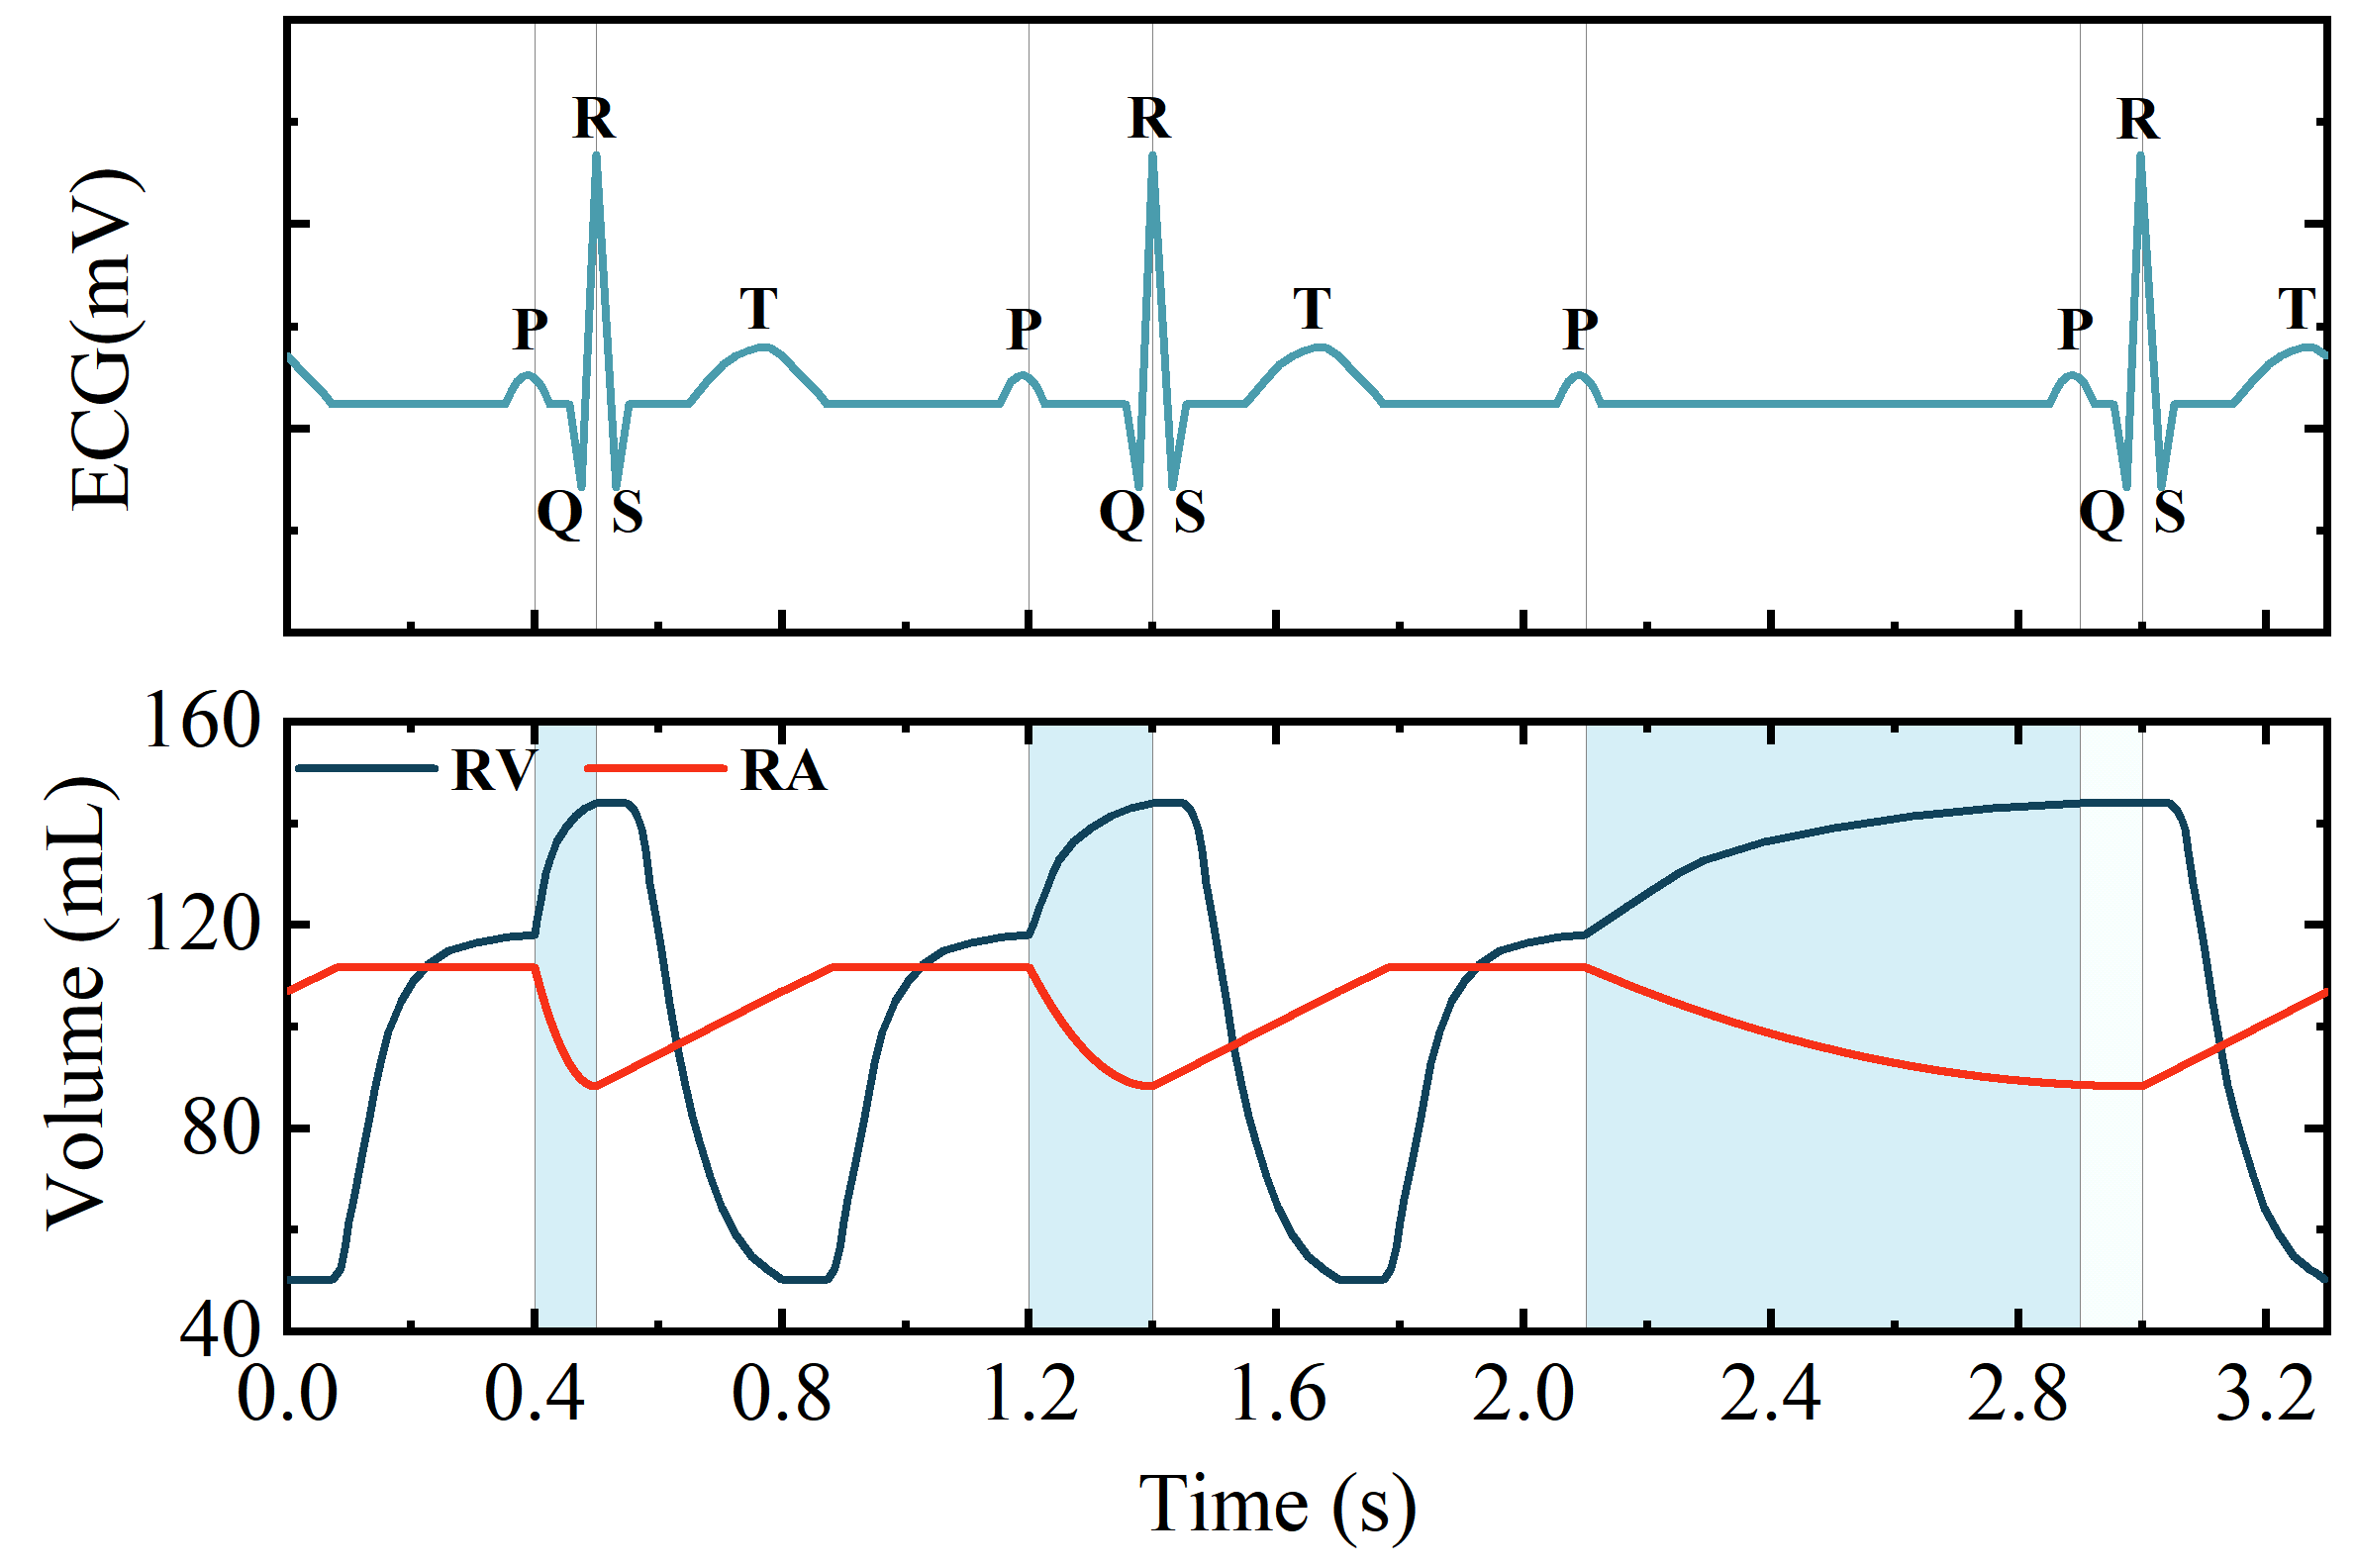
\includegraphics[width=0.9\columnwidth]{Figure/AVB_Vol}
    \caption{Pathological cardiac cycle simulation corresponding to our representative Atrioventricular Block (AVB) model. The map illustrates an instance of intermittent conduction failure, where a P-wave is not followed by a QRS complex, leading to an irregular hemodynamic profile.}
    \label{fig:avb_mapping}
\end{figure}




\begin{figure}[!t]
    \centering
    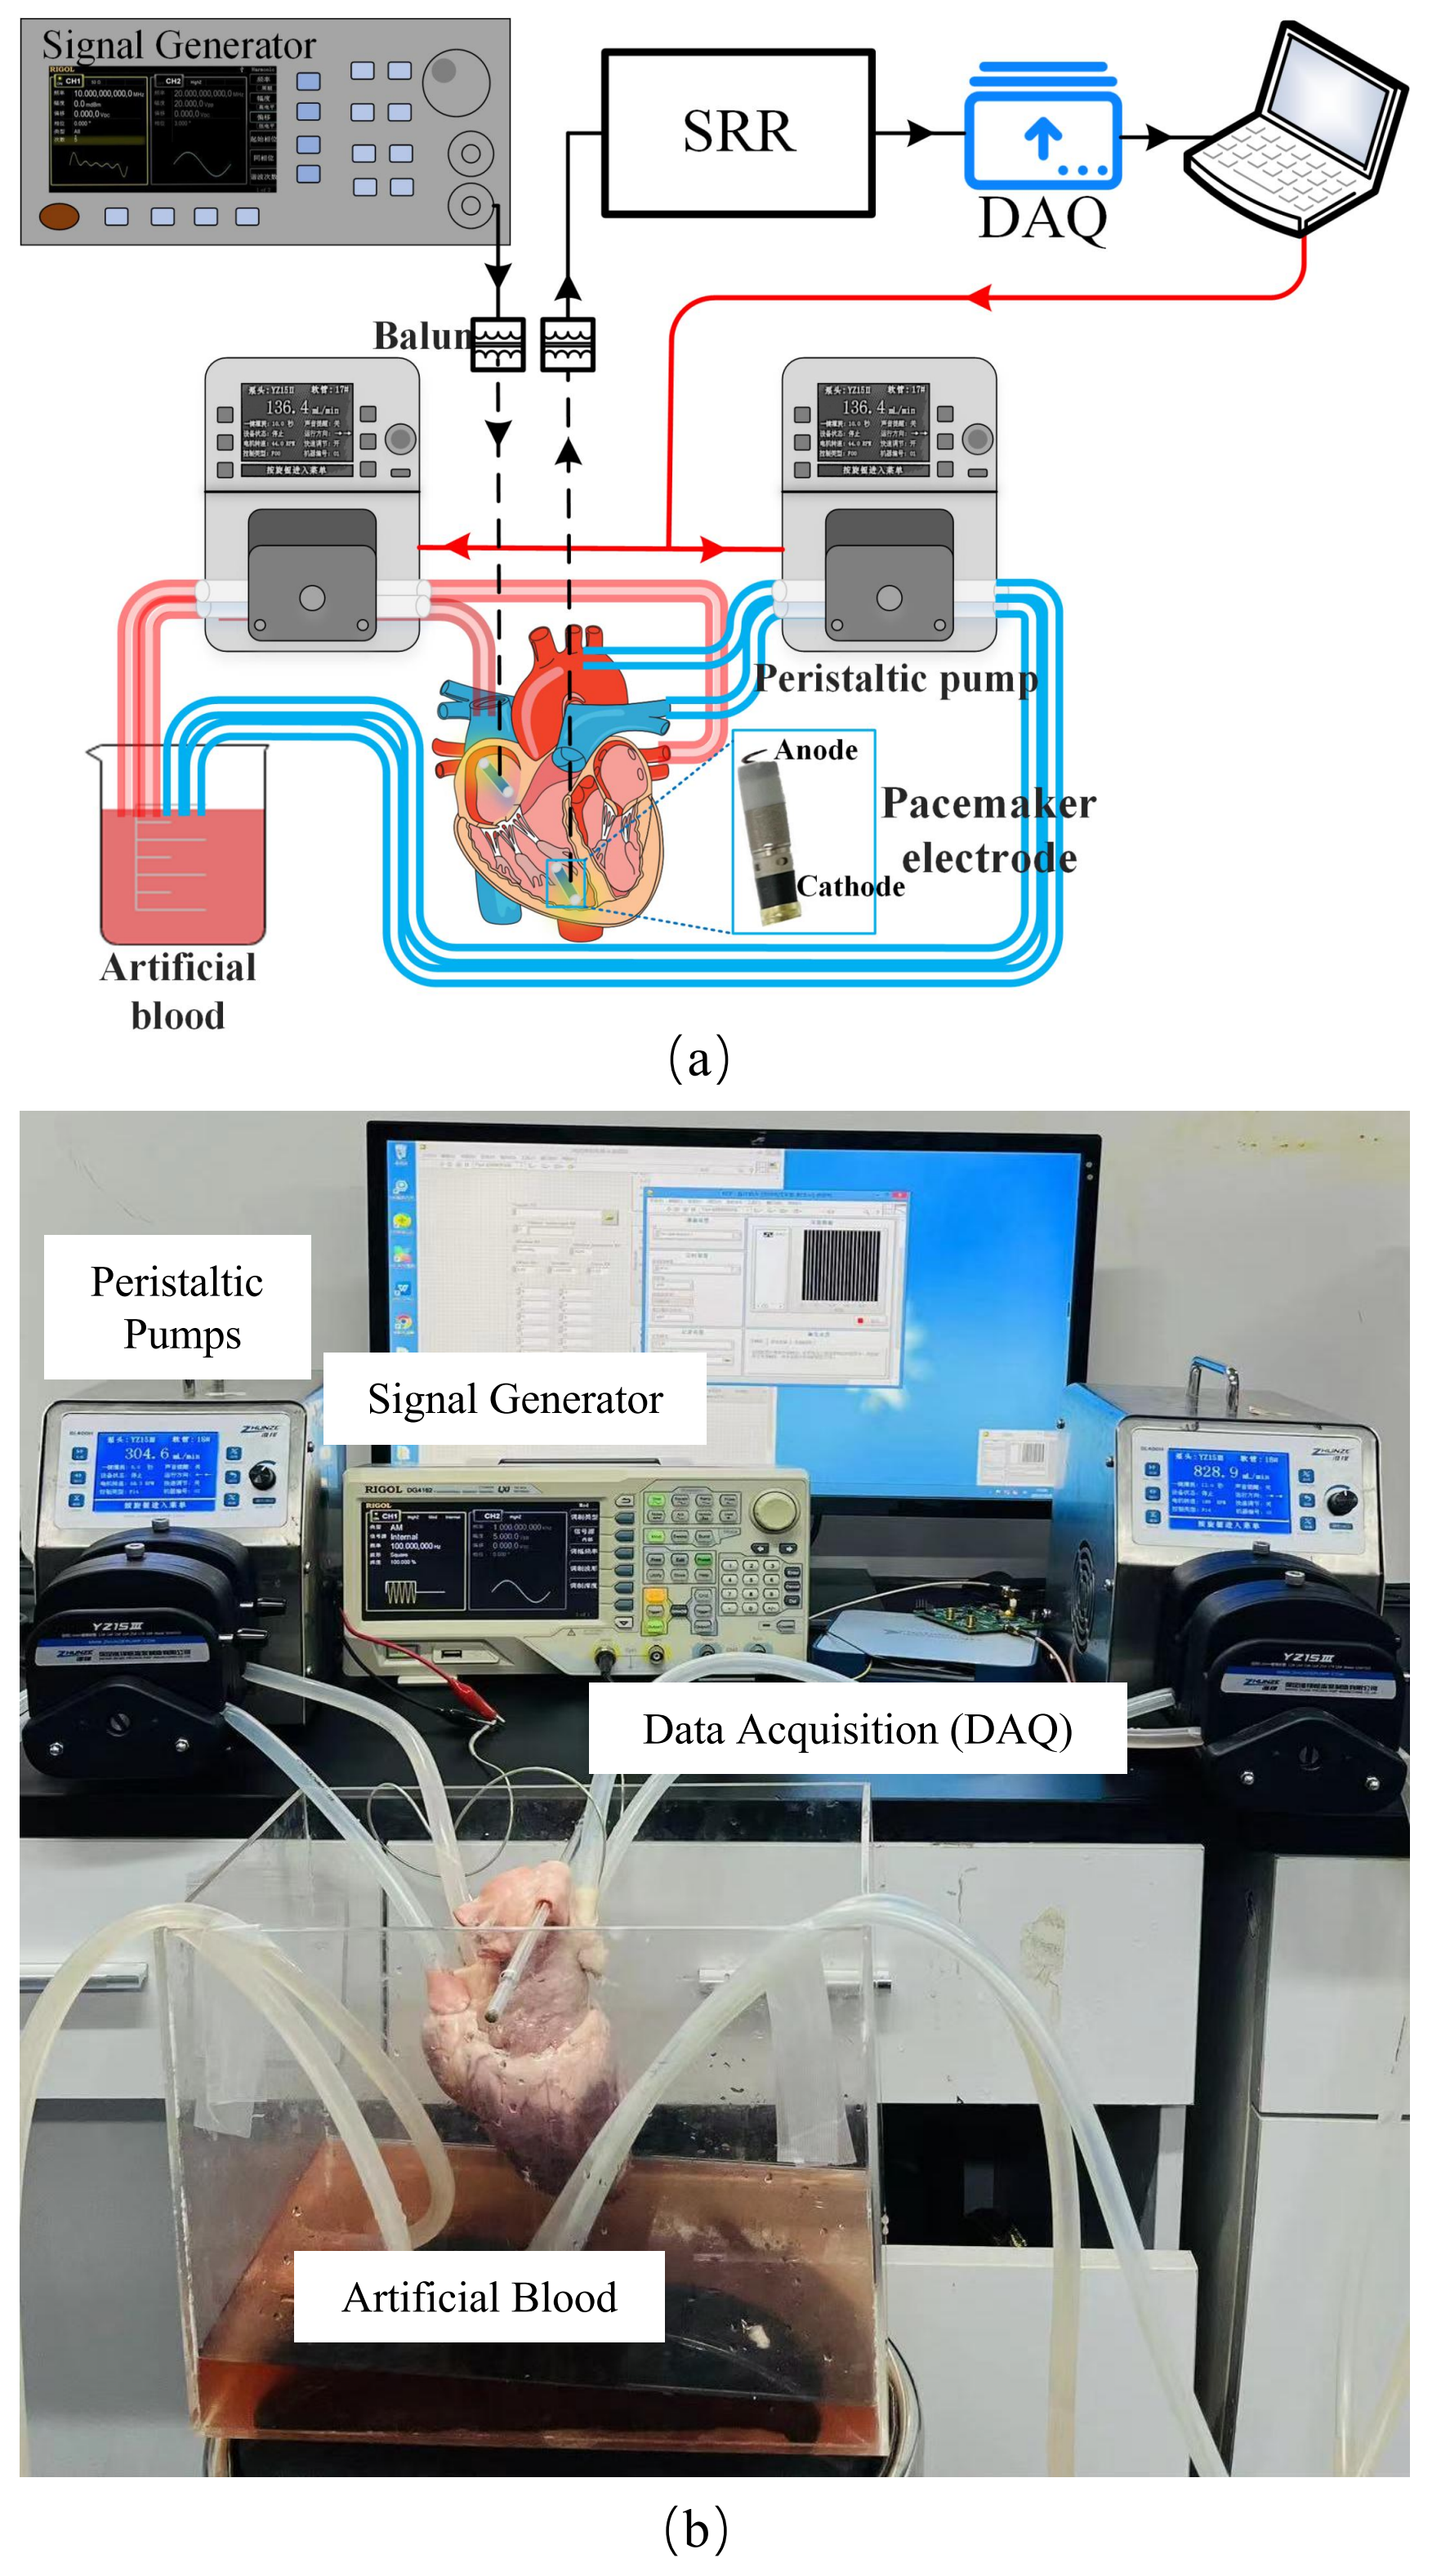
\includegraphics[width=0.95\columnwidth]{Figure/Mea_BER}
    \caption{Schematic of the experimental setup for BER evaluation. The configuration integrates a signal generator (SG), the \textit{ex-vivo} heart platform, the adaptive SRR, and a data acquisition (DAQ) system.}
    \label{BER}
\end{figure}


\section{Experimental Results and Analysis}
\label{sec:results}

A series of systematic ex-vivo experiments were conducted to comprehensively evaluate the proposed adaptive receiver architecture and its core 2-DOF control strategy.
This section sequentially constructs a complete argumentative chain: first, by presenting the true characteristics of the dynamic intracardiac channel, we reveal and quantify the core challenges of this research; second, we demonstrate the fundamental necessity of a basic AGC loop as a countermeasure; finally, through rigorous comparison with a traditional PID baseline, we will demonstrate the superior performance of our proposed 2-DOF controller in achieving robust communication from both transient response and statistical perspectives.


\subsection{Characterization of Channel Dynamics under Healthy and Pathological Rhythms}

Direct experimental characterization of the RA-RV intracardiac communication channel, as depicted in Fig.~\ref{fig:path_gain_variation}, reveals its inherent dynamic properties, providing a clear rationale for the design of an adaptive receiver.
Under simulated healthy heart conditions which is shown Fig.~\ref{fig:path_gain_variation}(a), the channel path gain exhibits pronounced yet highly periodic fluctuations of up to 10--15 dB, tightly synchronized with the cardiac cycle.
This baseline dynamic makes it clear that even under ideal conditions, a static receiver cannot guarantee stable communication quality, thus establishing the fundamental necessity for employing AGC.

However, the core challenge of this research is fully manifested when simulating pathological conditions.
As shown in Fig.~\ref{fig:path_gain_variation}(b), under the Mobitz Type I AVB model, the predictable rhythm of the channel is completely disrupted.
It is replaced by a harsh environment dominated by irregular, abrupt, and deep signal fades.
This qualitative shift from periodic fluctuations to unpredictable, event-driven transients imposes requirements on the adaptive system that are far beyond the conventional.
It indicates that a traditional feedback controller, which merely reacts to errors, will inevitably suffer from performance degradation when coping with such sudden fades.
Therefore, to maintain robust communication link integrity under these extreme conditions, an advanced control strategy capable of predictive and rapid response becomes essential.

\begin{figure}[!t]
    \centering
    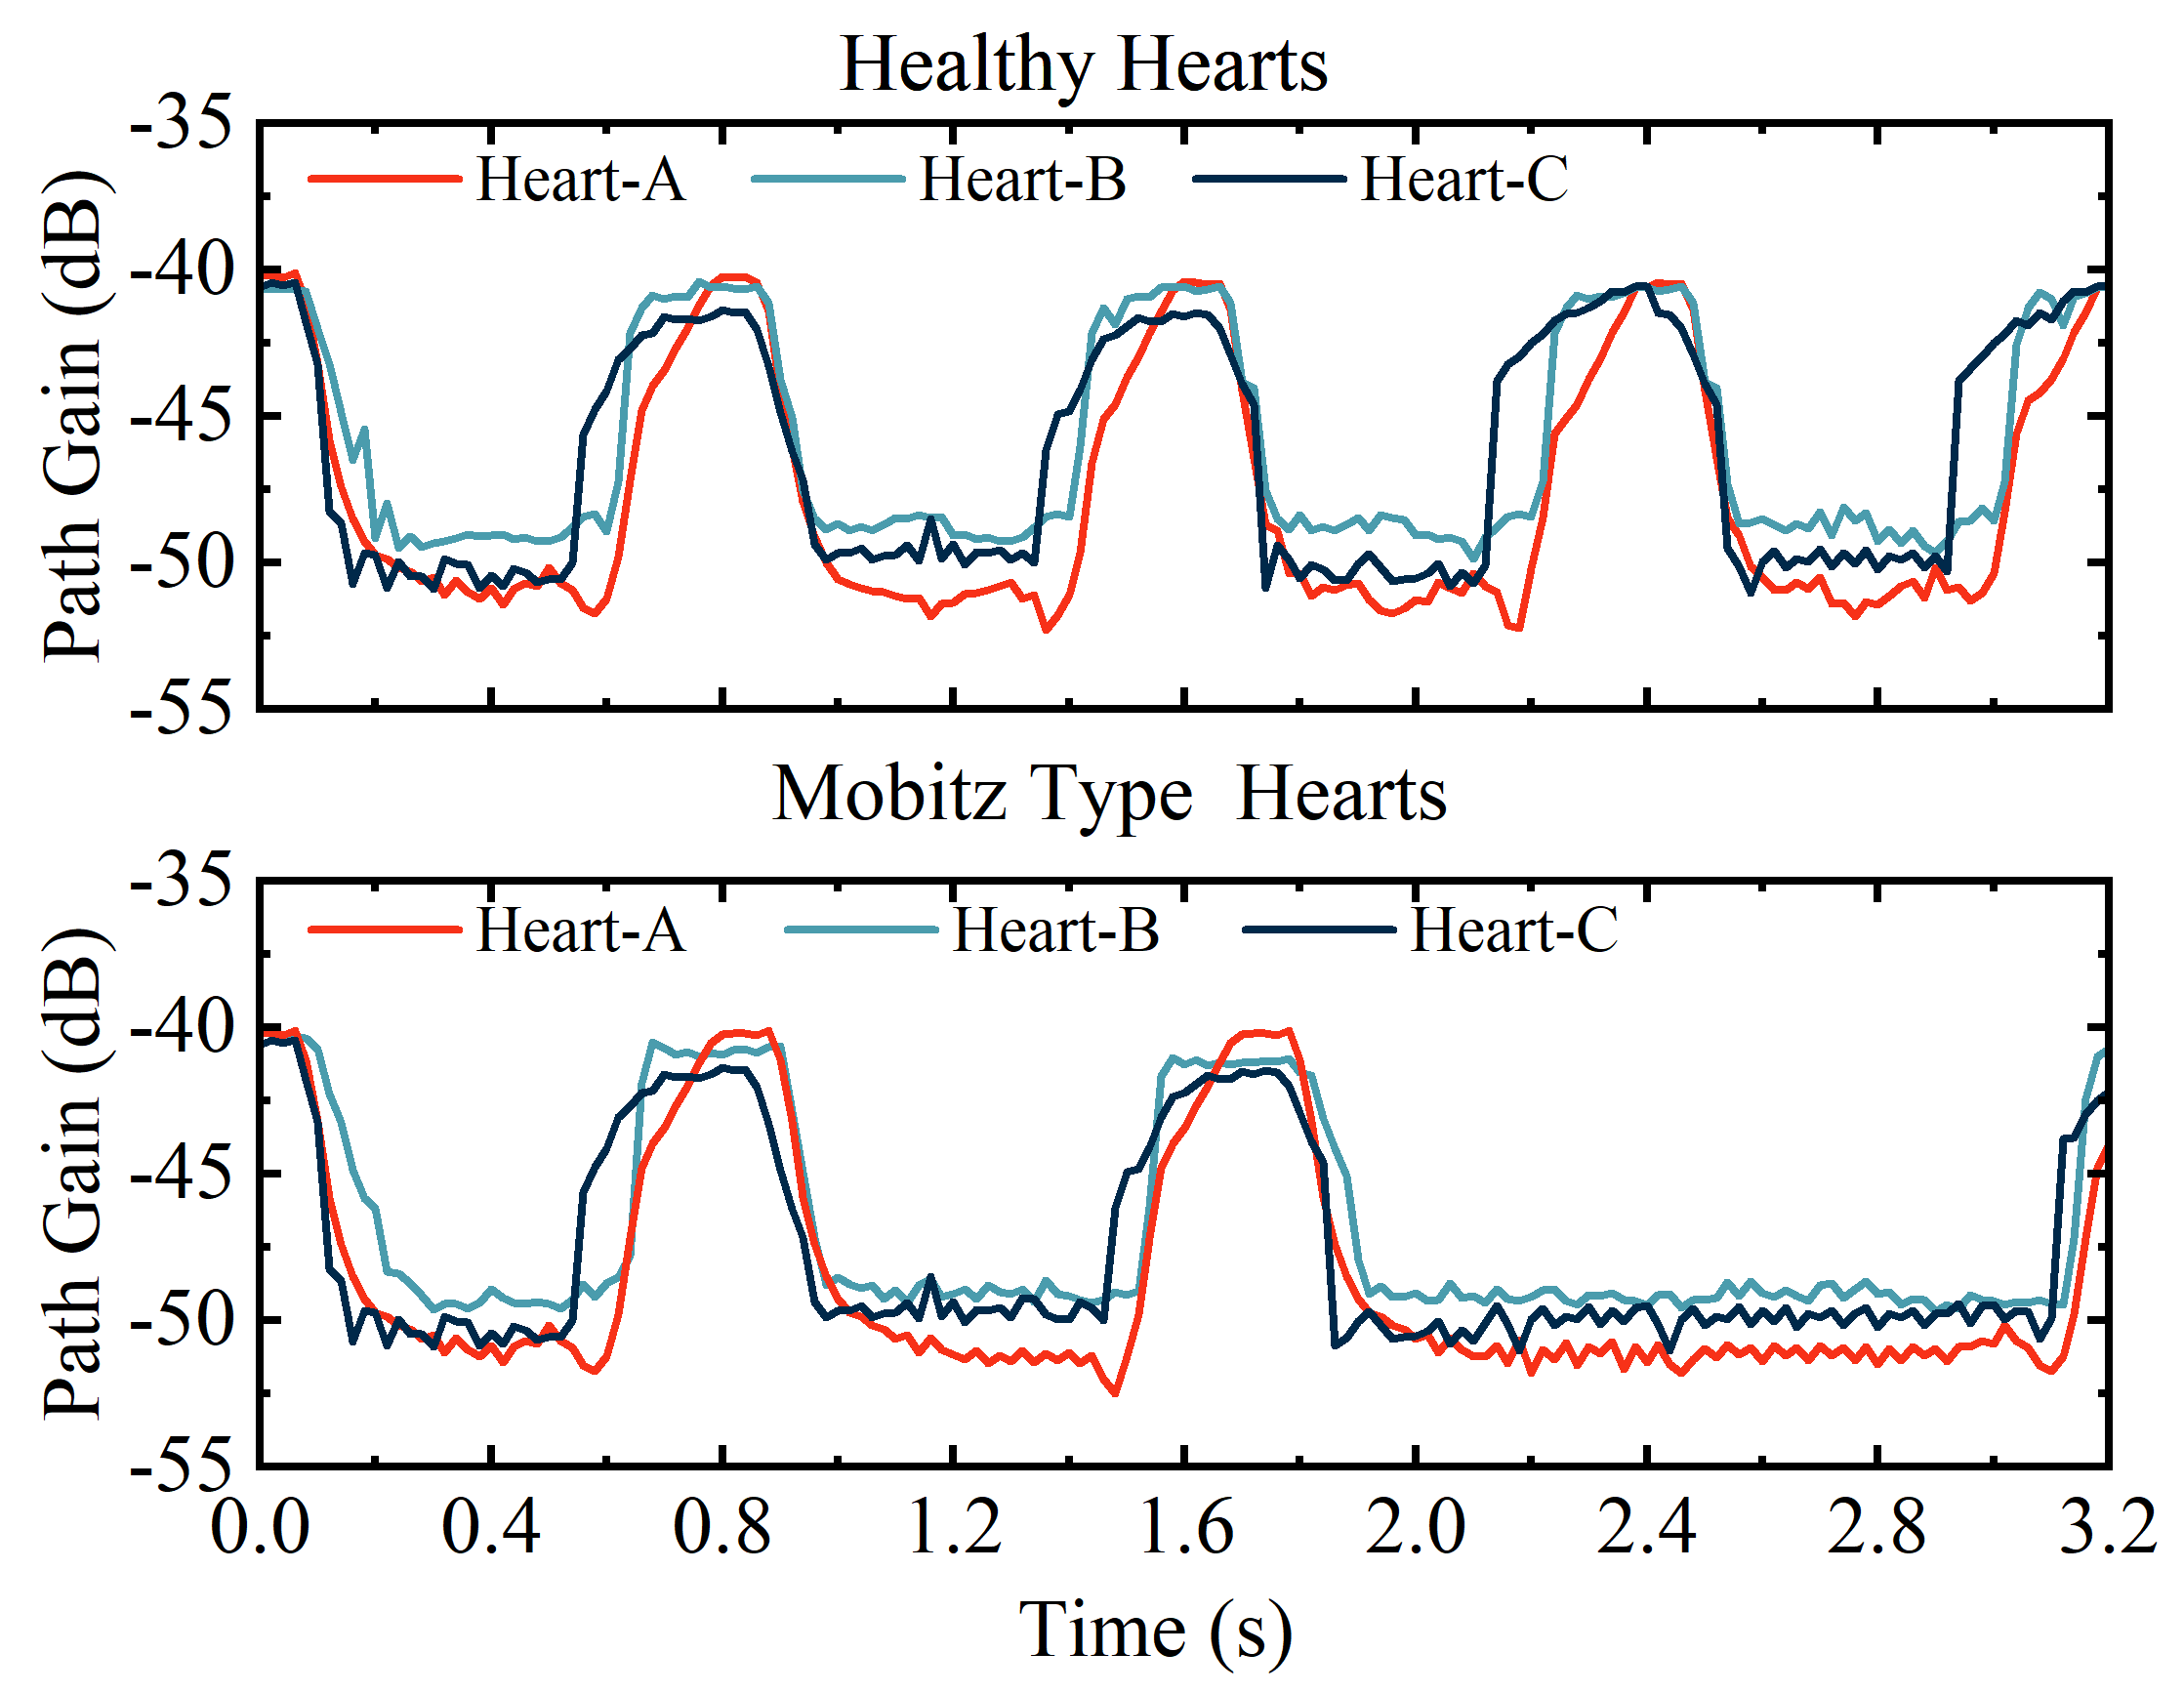
\includegraphics[width=0.9\linewidth]{Figure/signal_heart}
    \caption{Dynamic path gain variation of the RA-RV intracardiac channel. (a) Under simulated healthy heart conditions. (b) Under simulated representative pathological (Mobitz Type I AVB conditions. Results from three different ex-vivo porcine heart preparations are shown.}
    \label{fig:path_gain_variation}
\end{figure}


\subsection{Fundamental Effectiveness of the AGC System in Signal Stabilization}

Before introducing the advanced 2-DOF controller, we first had to establish the fundamental effectiveness of the AGC closed-loop itself as a solution. The basic capability of the AGC loop in stabilizing the severe channel fluctuations caused by heartbeats is illustrated in Fig.~\ref{fig:agc_effectiveness}, which uses the simulated pathological ECG in Fig.~\ref{fig:agc_effectiveness}(a) as a temporal reference.

The waveform in Fig.~\ref{fig:agc_effectiveness}(b) reveals the inherent instability without AGC, where the signal amplitude at the SRR input fluctuates drastically between 1.5~mV and 5.0~mV with the simulated heartbeats; this would directly translate into deteriorated demodulation performance. In stark contrast, when the AGC loop is activated, the VGA's control voltage ($V_g$) accurately tracks the channel variations in real-time and in an inverse manner, as depicted in the trace of Fig.~\ref{fig:agc_effectiveness}(c). The direct result, visualized in the stabilized waveform of Fig.~\ref{fig:agc_effectiveness}(d), is that the SRR's input signal amplitude is successfully clamped at the 100~mV target level, with peak-to-peak residual fluctuations suppressed to within 1\%. This result provides decisive evidence for AGC as a necessary technique to compensate for the dynamic channel.


\begin{figure}[!t]
    \centering
    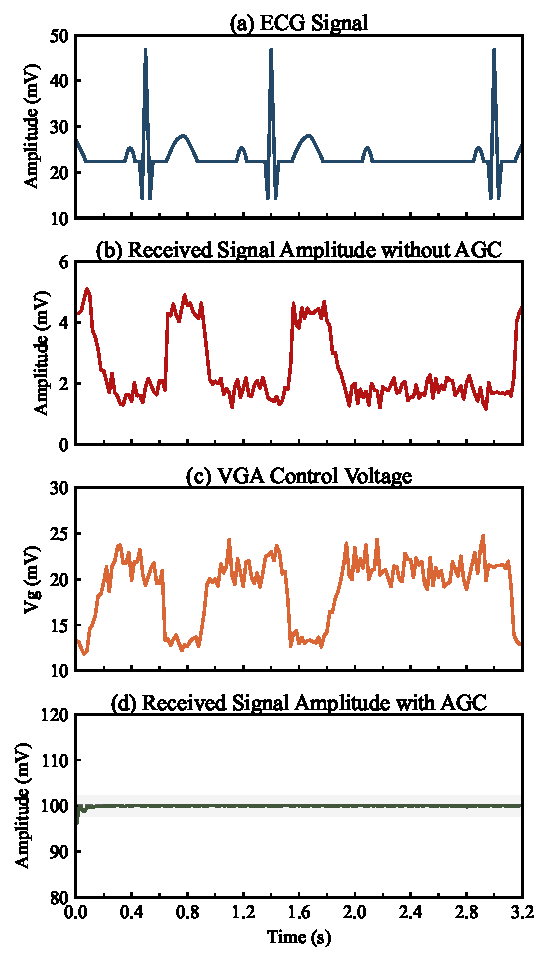
\includegraphics[width=0.9\linewidth]{Figure/agc}
    \caption{Effectiveness of the hybrid AGC system in stabilizing the receiver input signal. (a) Reference ECG signal. (b) Received signal amplitude at the SRR input without AGC. (c) Dynamic VGA control voltage ($V_g$). (d) Stabilized signal amplitude at the SRR input with AGC activated.}
    \label{fig:agc_effectiveness}
\end{figure}



\subsection{Comprehensive Evaluation of Transient Response Performance}

To quantify the advantages of our proposed 2-DOF strategy over a traditional PID baseline, we evaluated the transient response of the AGC control algorithm under a challenging 15 dB channel step event. The results, depicted in Fig.~\ref{fig:transient_response}, reveal a stark performance difference. Following a sharp drop in channel gain, the feedback-only PID controller shows significant undershoot, with its signal amplitude falling to 87.7\% of its target, representing a maximum deviation of 12.3\%, and requiring 85.2 ms to re-settle. Conversely, thanks to its predictive feedforward path, the 2-DOF controller restricts the maximum deviation to only 9.1\% and maintains the signal above 90.9\% of its target value. It also dramatically reduces the settling time to just 20.3 ms, which is a greater than four-fold, or 76\%, improvement over the baseline.


To generalize this significant advantage from a representative event to a statistically meaningful conclusion, we further performed an aggregate analysis of key dynamic performance metrics measured across repeated experiments under various disturbance scenarios, with the results presented in Fig.~\ref{fig:quantitative_transient}. The statistical results irrefutably confirm the comprehensive superiority of the 2-DOF controller in dynamic performance, especially in response speed.

The statistical results for settling time, presented in Fig.~\ref{fig:quantitative_transient}(a), highlight a compelling advantage of the 2-DOF architecture, which reduces the settling time by more than 4 times, a reduction of approximately 76\%, across all tested scenarios. This superior performance extends to the suppression of maximum deviation, where the data in Fig.~\ref{fig:quantitative_transient}(b) shows a consistent improvement that reduces the deviation by about 20--26\% in all scenarios. Thus, the combined evidence from the in-depth analysis of a single typical event and this broader cross-scenario statistical validation robustly proves that the 2-DOF architecture possesses far superior speed and stability in coping with channel transients compared to traditional feedback control.



\begin{figure}[!t]
    \centering
    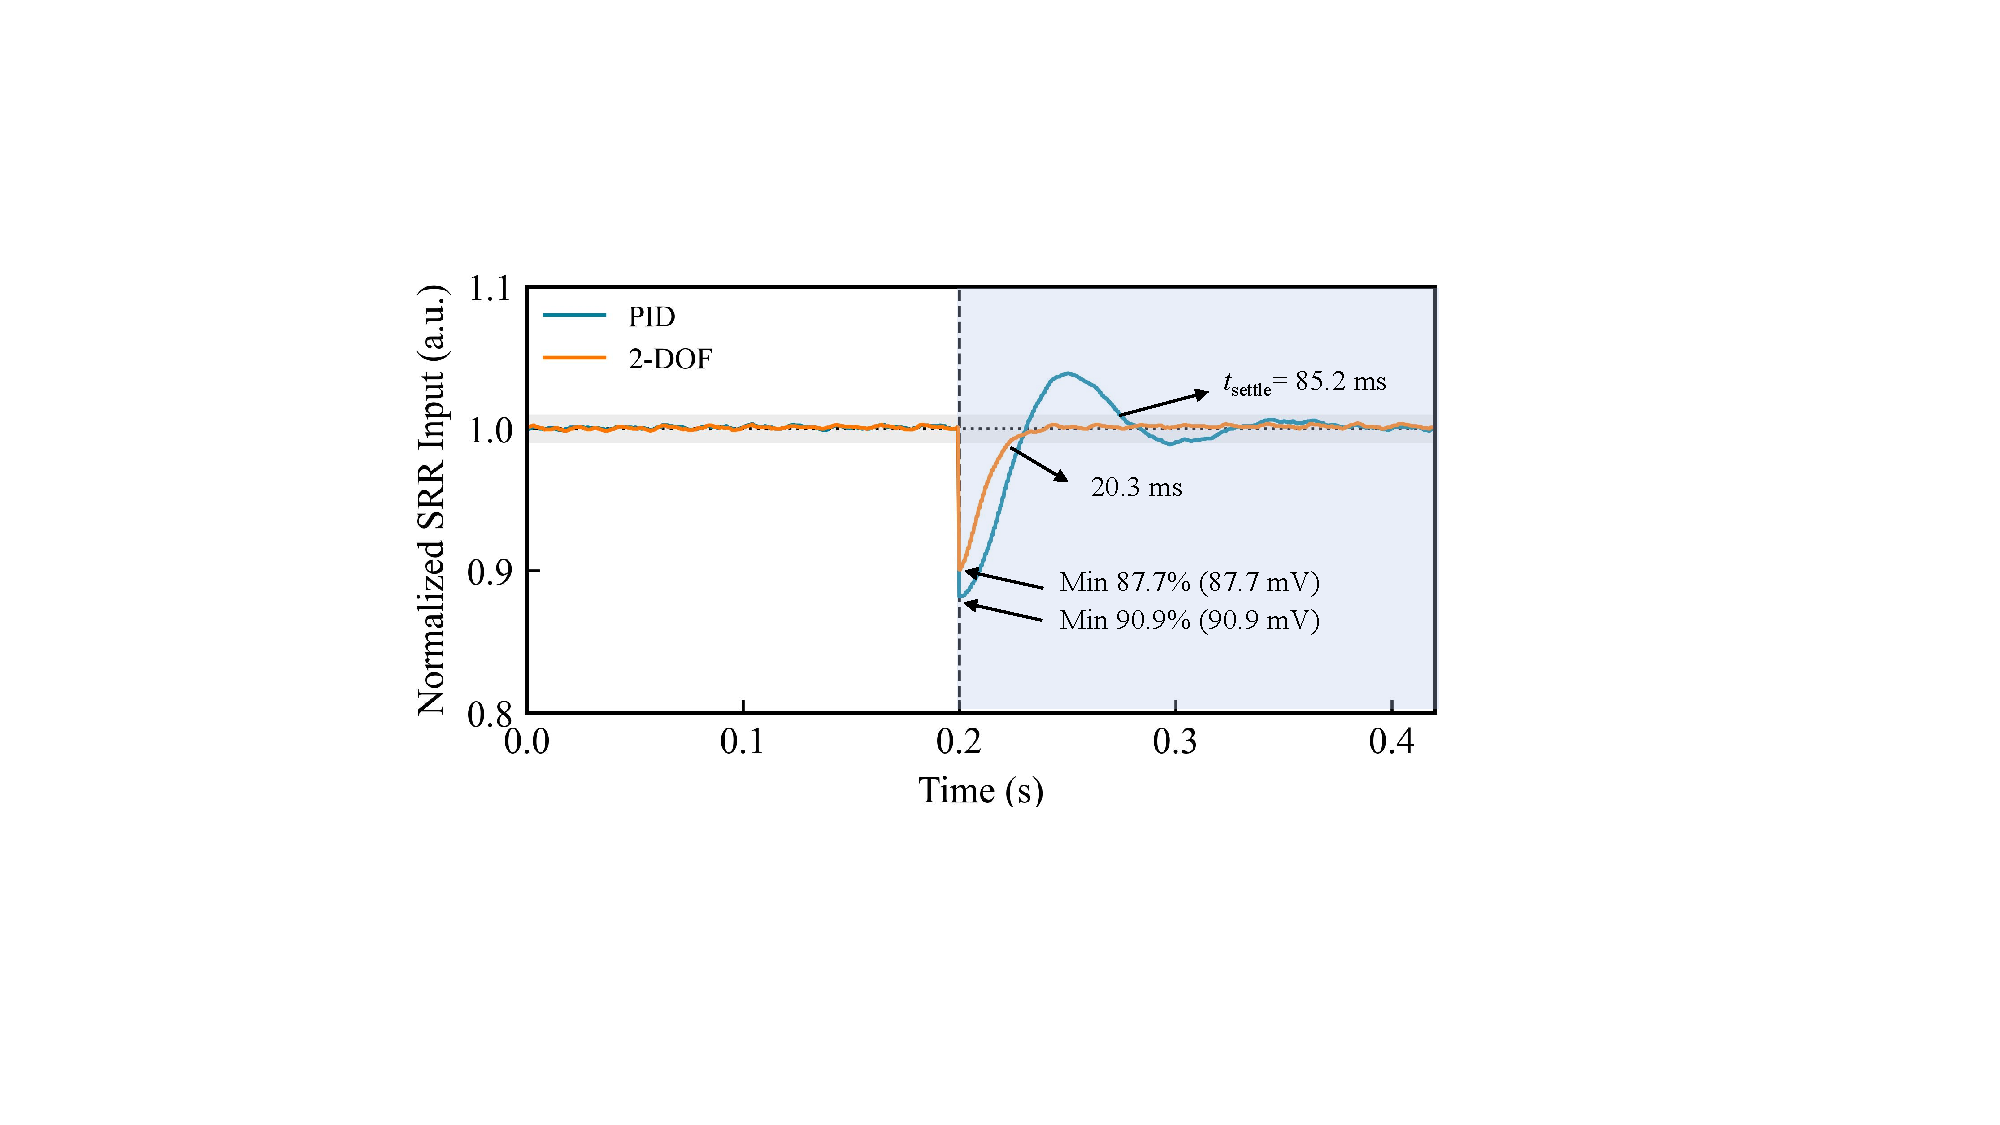
\includegraphics[width=9cm]{Figure/step}
    \caption{Transient response comparison between the 2-DOF and PID controllers to a representative 15\,dB channel gain step. The normalized SRR input signal demonstrates the superior performance of the 2-DOF controller in terms of both settling time and undershoot suppression.}
    \label{fig:transient_response}
\end{figure}



\begin{figure}[!t]
    \centering
    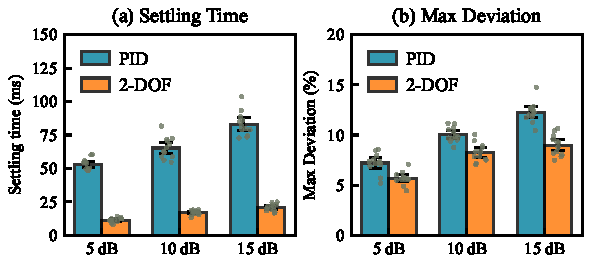
\includegraphics[width=8.5cm]{Figure/R2_step_bar}
  \caption{Quantitative statistical comparison of transient performance metrics under different channel step disturbances. (a) Settling time ($t_{\text{settle}}$) comparison. (b) Maximum deviation (\%) comparison. Data points represent individual trials, while bars and error whiskers indicate the mean and 95\% confidence interval, respectively. The 2-DOF controller significantly outperforms the baseline PID across all scenarios.}
    \label{fig:quantitative_transient}
\end{figure}




\subsection{Final Enhancement in Communication Reliability}

The ultimate value of superior signal stability must be manifested in an improvement in actual communication performance. Fig.~\ref{fig:ook_demodulation} first visually demonstrates the AGC system's assurance of signal integrity in the time domain. Even under a dynamic channel, the envelope of the received OOK signal is maintained at a constant level, ensuring that the subsequent demodulation circuit can flawlessly recover the original baseband signal.

We quantified the final communication performance by the Bit Error Rate (BER), with the results presented in Fig.~\ref{fig:ber_vs_datarate}. The experimental results provide compelling evidence for the decisive role of adaptive control. Compared to the configuration without AGC, both AGC strategies (PID and 2-DOF) substantially reduced the BER across all tested data rates, with the 2-DOF configuration achieving an average improvement of 98.4\% at a 5\,kbps data rate.

More importantly, the data further reveals the significant superiority of our proposed 2-DOF controller over the conventional PID baseline. Across all data rates, the 2-DOF controller consistently achieved a lower BER. This advantage becomes dramatically more pronounced as the data rate increases, highlighting its resilience to inter-symbol interference. For instance, while the performance improvement factor of the 2-DOF controller over the No-AGC case is approximately 24-fold at 500\,bps, this factor escalates to over 63-fold at 5\,kbps. At this highest tested data rate, the 2-DOF controller reduced the average BER from the PID's $9.0 \times 10^{-5}$ down to $1.5 \times 10^{-5}$, representing an additional 83.3\% error rate reduction on top of the already-optimized PID. This trend unequivocally demonstrates that the superior transient response of the 2-DOF controller translates into exceptional robustness for high-speed communication. Therefore, the proposed adaptive receiver architecture provides a key technical foundation for ensuring high-reliability communication for LCPs in complex pathological environments.


\begin{figure}[!t]
    \centering
    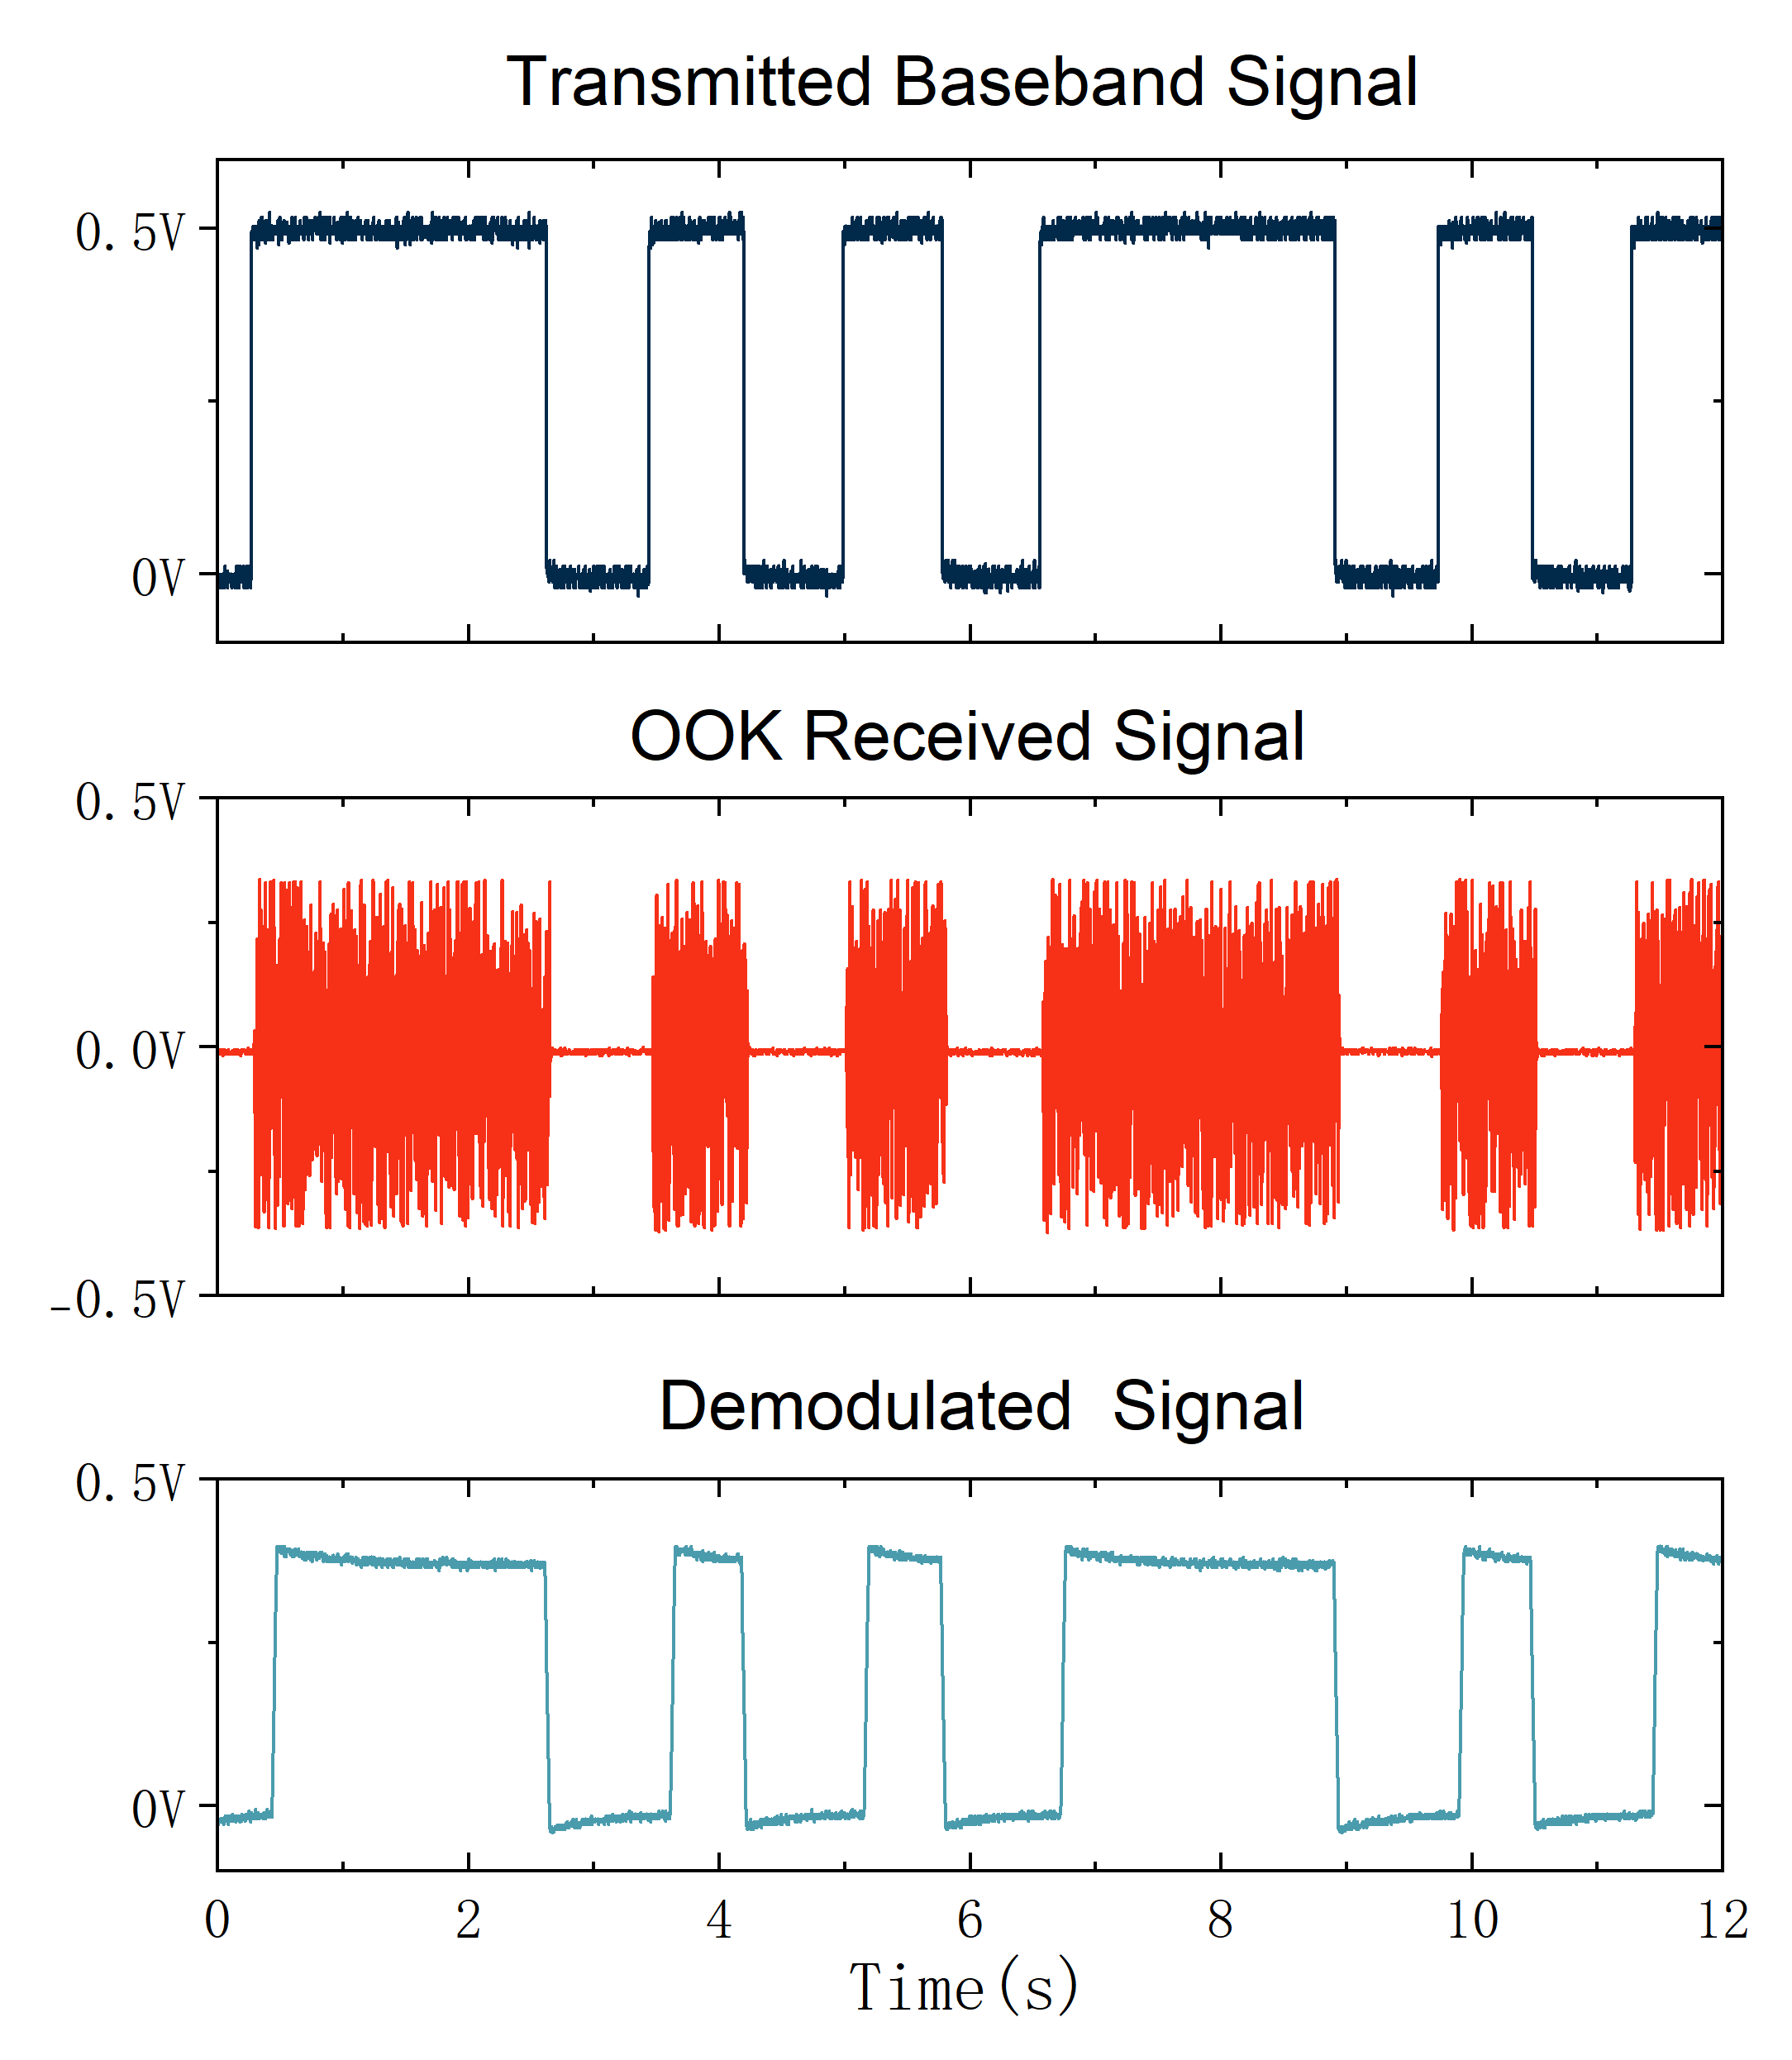
\includegraphics[width=0.8\linewidth]{Figure/ook}
    \caption{OOK signal waveforms at different stages of the system with AGC activated. (a) Transmitted baseband signal. (b) Received signal at the SRR input. (c) Demodulated baseband signal at the SRR output.}
    \label{fig:ook_demodulation}
\end{figure}


\begin{figure}[!t]
    \centering
    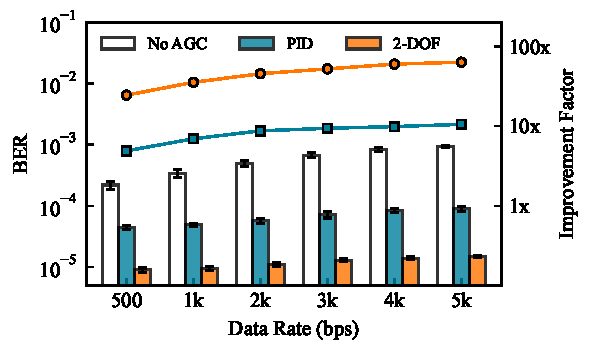
\includegraphics[width=0.95\linewidth]{Figure/ber}
   \caption{BER performance comparison for No-AGC, PID, and 2-DOF configurations across various data rates under the simulated pathological condition. The plot highlights the significant BER reduction achieved by AGC, with the 2-DOF controller demonstrating superior performance over the traditional PID. Error bars represent the standard deviation across N=3 independent heart preparations.}
    \label{fig:ber_vs_datarate}
\end{figure}


\begin{table*}[htbp]
\centering
\caption{Performance Comparison with Related Receiver Prototypes}
\label{tab:comparison}
\begin{tabularx}{\textwidth}{l >{\raggedright\arraybackslash}X >{\raggedright\arraybackslash}X >{\raggedright\arraybackslash}X >{\raggedright\arraybackslash}X >{\raggedright\arraybackslash}X}
\toprule
Metric & Bereuter et al.~\cite{bereuter2019leadless} & Ryser et al.~\cite{ryser2022modulation} & Khaleghi et al.~\cite{khaleghi2020conductive} & Yuk et al.~\cite{yuk2020implantable} & This Work \\
\midrule
Primary focus & In-vivo channel characterization & Modulation scheme analysis & Broadband channel modeling & Low-power integrated circuit & Pathological channel robustness \\
\addlinespace
Measurement Type & In-vivo & Ex-vivo & Ex-vivo & In-vivo/Ex-vivo & Ex-vivo \\
\addlinespace
Frequency [MHz] & 1 & 1.5 & 0.01-10 & DC-20 & 1 \\
\addlinespace
Receiver Power [mW] & $>$465 & 152 & 230 & 0.062 & 268 \\
\addlinespace
Technology & Discrete components & Discrete components & Discrete components & 110nm CMOS & Discrete components \\
\midrule % Added a midrule for visual separation of the new section
NSR Dynamics  & \times & \times & \times & \times & \checkmark \\
\addlinespace
Pathological Dynamics  & \times & \times & \times & \times & \checkmark \\
\addlinespace
Adaptive Gain Compensation & \times & \times & \times & \times & \checkmark \\
\bottomrule
\end{tabularx}
\end{table*}

\section{Discussion}
\label{sec:discussion}

This study was centered on the core challenge of robust intracardiac communication under pathological cardiac rhythms. Experimental results demonstrate that the proposed adaptive receiver maintains a stable signal amplitude and significantly reduces the bit error rate, even in the presence of abrupt and unpredictable channel gain jumps triggered by events such as Atrioventricular block. This highlights a key shift in design philosophy: intracardiac communication systems must evolve from adapting to regular, healthy rhythms to actively tracking and suppressing aperiodic, pathologically-driven events. Our beat-synchronous 2-DOF strategy achieves this by using the RSSI as an ECG-free proxy for the cardiac rhythm, enabling beat-by-beat prediction and feedforward presetting, which is complemented by an incremental PID to suppress intra-beat residual errors. This ``predict and correct" combination allows the system to maintain a stable demodulation boundary during sudden transients.

As summarized in Table~\ref{tab:comparison}, this work's starting point and evaluation scenario are more aligned with clinical reality compared to prior art~\cite{bereuter2019leadless,ryser2022modulation,khaleghi2020conductive,yuk2020implantable}.
Previous research has largely focused on channel characterization, modulation analysis, or broadband modeling, almost entirely under static or quasi-static assumptions.
While excellent progress has been made in low-power integrated circuit implementation, systematically addressing the communication robustness challenges posed by cardiac dynamics, especially pathological dynamics, remains an open problem.
This work focuses on this ``pathological channel robustness" gap by advancing the evaluation scenario from static to dynamic, and further to pathological conditions. As Table~\ref{tab:comparison} also makes clear, existing prototypes generally lack adaptive gain compensation for dynamic channels.
In contrast, the hybrid architecture and beat-synchronous prediction proposed here are designed to balance response speed and steady-state performance in a highly time-varying channel, directly filling this critical technological gap.

The proposed method, being designed for event-driven aperiodic transients, is expected to be extensible to other scenarios such as dropped beats, intermittent conduction abnormalities, and highly irregular intervals. It should be noted that the current ex vivo platform cannot cover all in-vivo complexities, such as autonomic nervous regulation, long-term tissue-electrode interface changes, and respiratory coupling. The prototype was also implemented with discrete components to validate the control concept and architecture, rather than as a final implantable device.

From a clinical perspective, reliable intracardiac communication is fundamental for synchronized pacing and inter-chamber coordination in multi-chamber pacemaker systems. In settings dominated by pathological rhythms, the ability to proactively preset the gain and rapidly stabilize the link helps ensure the accurate delivery of rhythm management and therapeutic sequences. Future work will focus on the CMOS integrated circuit implementation of this architecture, balancing low latency with fixed-point complexity while ensuring stability margins. This will be followed by longer-term large-animal in-vivo studies covering a broader range of pathological types and more complex physiological conditions to further validate the method's transferability and long-term stability.

%本研究围绕病理性心律下心脏内稳健通信这一核心挑战展开。实验结果表明，所提出的自适应接收器即使在房室传导阻滞等事件引发的突发且不可预测的信道增益跳变情况下，仍能保持稳定的信号幅度，并显著降低误码率。这凸显了设计理念的一个关键转变：心内通信系统必须从适应规律的健康心律，转变为主动跟踪和抑制非周期性、由病理驱动的事件。我们的心跳同步双自由度（2-DOF）策略通过将接收信号强度指示器（RSSI）用作无需心电图（ECG）的心脏节律替代指标来实现这一点，从而能够进行逐跳预测和前馈预置，并辅以增量式比例-积分-微分（PID）控制器来抑制跳内残留误差。这种“预测与校正”相结合的方式使系统在突发瞬变期间能够维持稳定的解调边界。
%
%如表\ref{tab:comparison}所总结，与先前的研究相比，本研究的起点和评估场景更贴合临床实际。以往的研究主要集中在信道表征、调制分析或宽带建模上，且几乎都是在静态或准静态假设下进行的。尽管在低功耗集成电路实现方面取得了显著进展，但系统地解决心脏动态（尤其是病理性动态）带来的通信稳健性挑战仍是一个尚未解决的问题。本研究通过将评估场景从静态推进到动态，进而到病理状态，聚焦于这一“病理信道稳健性”空白。如表\ref{tab:comparison}所示，现有原型通常缺乏针对动态信道的自适应增益补偿。相比之下，本文提出的混合架构和心跳同步预测旨在平衡高时变信道中的响应速度和稳态性能，直接填补了这一关键技术空白。
%
%所提出的方法专为事件驱动的非周期性瞬变而设计，有望扩展到其他场景，如心跳脱落、间歇性传导异常和高度不规则的间隔等。需要注意的是，当前的离体平台无法涵盖所有在体复杂性，例如自主神经调节、长期组织-电极界面变化以及呼吸耦合等。该原型也是采用分立元件实现的，目的是验证控制概念和架构，而非作为最终的可植入设备。
%
%从临床角度来看，可靠的心脏内通信是多腔室起搏器系统中同步起搏和心腔间协调的基础。在以病理性心律为主的情况下，主动预置增益和快速稳定链路的能力有助于确保节律管理和治疗序列的准确传递。未来的工作将集中在该架构的互补金属氧化物半导体（CMOS）集成电路实现上，在平衡低延迟与定点复杂性的同时确保稳定性裕度。随后，将进行长期的大型动物在体研究，涵盖更广泛的病理类型和更复杂的生理条件，以进一步验证该方法的可转移性和长期稳定性。


\section{Conclusion}
\label{sec:conclusion}

This paper addressed the critical challenge of maintaining robust intracardiac communication amidst the unpredictable channel fades caused by pathological cardiac events. To overcome the limitations of conventional reactive control, we proposed and validated a novel adaptive receiver architecture featuring a beat-synchronous, 2-DOF Hybrid-AGC controller that proactively compensates for channel variations by using the RSSI as an ECG-free proxy for the cardiac rhythm. Systematic evaluation demonstrated that the controller stabilizes the received signal to within 1\% of its target despite channel gain fluctuations exceeding 15\,dB. This stabilization translates into a bit error rate improvement of up to 98.4\%, which corresponds to a reliability enhancement factor of over 60. This research, therefore, delivers not only a key enabling technology for clinically reliable LCP systems but also offers a rigorously validated and generalizable design paradigm for the next generation of networked IMDs intended to operate robustly in harsh biological environments.

\bibliographystyle{ieeetr}
\bibliography{Reference}



\begin{IEEEbiography}
[{
\includegraphics[width=1in,height=1.25in,clip,keepaspectratio]{Figure/author/Dongming Li.png}}]
{Dongming Li}(Student Member, IEEE) received the M. S. degree in the College of Physics and Information Engineering from Fuzhou University, Fuzhou, China, in 2021.
He is currently pursuing the Ph.D.\ degree in the State Key Laboratory of Analog and Mixed-Signal VLSI, University of Macau. His current research interests include biomedical Integrated circuits, miniaturized sensors for biomedical applications, Leadless pacemaker intracardiac communication, and human body communication.
\end{IEEEbiography}

\vspace{10mm}
\begin{IEEEbiography}[{
\includegraphics[width=1in,height=1.25in,clip,keepaspectratio]{Figure/author/Yu_Xia}}]
{Yu Xia} (Student Member, IEEE) received the M.S. degree in 2024 from the Department of Electrical and Computer Engineering, University of Macau, Macau, where he is currently working toward the Ph.D. degree in the University of Macau and the KU Leuven. His research interests include ASIC，Low noise amplifier, neural AFE, biomedical signal acquisition, pseudo-resistor, and electrical impedance measurement.
\end{IEEEbiography}
\vspace{10mm}

\begin{IEEEbiography}
[{
\includegraphics[width=1in,height=1.25in,clip,keepaspectratio]{Figure/author/Han Wang}}]
{Han Wang} received the B. S. degree from the College of Internet of Things Engineering Program, Fuzhou University, Fuzhou, China, in 2021.
He is currently working toward the Ph.D.\ degree with the College of Physical and Information Engineering, Fuzhou University, Fuzhou, China.
His research focuses on intrabody communication, biomedical signal detecting technology.
\end{IEEEbiography}
\vspace{10mm}


\begin{IEEEbiography}[{
\includegraphics[width=1in,height=1.25in,clip,keepaspectratio]{Figure/author/Sio Hang Pun.png}}]
{Sio Hang Pun} (Senior Member, IEEE) received his M. S. degree in Computer and Electrical program from the University of Porto, Portugal, 1999 and the Ph. D. Degree in the Electrical and Electronics Engineering from the University of Macau, Macau, 2012. Currently, he is an Associate Professor in the State Key Laboratory of Analog \& Mixed-Signal VLSI of the University of Macau. His current research interests include Biomedical Electronic Circuits, Miniaturized Sensors for Biomedical Applications and Human Body communication.
\end{IEEEbiography}

\begin{IEEEbiography}
[{
\includegraphics[width=1in,height=1.25in,clip,keepaspectratio]{Figure/author/Yueming Gao}}]
{Yueming Gao} (Senior Member, IEEE) received the Ph.D.\ degree in electrical engineering from Fuzhou University, Fuzhou, China, in 2010.
Since 2004, he has been involved in research in the areas of bioelectromagnetic and biomedical signal detecting technology.
He is currently a Professor in the College of Physical and Information Engineering, Fuzhou University.
\end{IEEEbiography}
\vspace{-10mm}


\vspace{10mm}
\begin{IEEEbiography}
[{
\includegraphics[width=1in,height=1.25in,clip,keepaspectratio]{Figure/author/Wangbin Ding}}]
{Wangbin Ding} (Member, IEEE) Wangbin Ding was born in Lishui City, Zhejiang Province, China in 1990.
He received his B.S. degree and M.Eng. degree in software engineering from Northwestern Polytechnical University, China, in 2012 and 2015, respectively.
He obtained his Ph.D. degree in Communication and Information Systems from Fuzhou University, China, in 2023.
He is currently an Lecturer at the Schoolof Medical Imaging, Fujian Medical University.
His primary research interests lie in medical image analysis, deep learning, and artificial intelligence.
\end{IEEEbiography}

\vspace{-10mm}
\begin{IEEEbiography}[{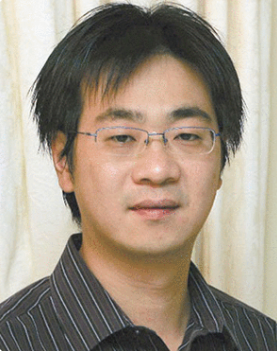
\includegraphics[width=1in,height=1.25in,clip,keepaspectratio]{Figure/author/liuyu}}]
  {Yu Liu} (Member, IEEE) received the B.Eng.
  degree in electronic engineering, the M.Eng.
  degree in information and communication engineering, and the Ph.D.\ degree in signal and information processing from Tianjin University, Tianjin, China, in 1998, 2002, and 2005, respectively.
  In 2000, he joined Tianjin University.
  Since 2008, he has been an Associate Professor with the School of Electronic and Information, Tianjin University.
  From 2011 to 2012, he was a Visiting Fellow with the Department of Electrical Engineering, Princeton University, Princeton, NJ, USA. His research interests include signal/video processing, medical signal processing, multimedia systems, compressed sensing, and indoor positioning systems.
\end{IEEEbiography}

\vspace{10mm}
\begin{IEEEbiography}
[{
\includegraphics[width=1in,height=1.25in,clip,keepaspectratio]{Figure/author/Hung Chun Li}}]
{Hung-Chun Li} received the Master of Science (M.Sc.) degree in electrical engineering from
National Taiwan University, Taipei, Taiwan, in 1990,and the master’s degree from the University of Florida, Gainesville, FL, USA, in 1994.
He is currently with the Joint Laboratory of Zhuhai UM Science and Technology Research Institute—Lingyange Semiconductor Incorporated,
Zhuhai, China.
\end{IEEEbiography}

\vspace{10mm}
\begin{IEEEbiography}
[{\includegraphics[width=1in,height=1.25in,clip,keepaspectratio]{Figure/author/anguo zhang}}]
{Anguo Zhang} (Senior Member, IEEE) Anguo Zhang was born in Hefei city, Anhui province, China in 1990.
 He received his B.S. degree in Automation and M.Eng. degree in Control Engineering from Chongqing University, China, in 2012 and 2016, respectively.
He obtained his Ph.D. degree in Communication and Information Systems from Fuzhou University, China, in 2022.
He is currently an Associate Professor at the Interdisciplinary Institute for Medical Engineering, Fuzhou University.
His primary research interests lie in brain-inspired neural networks, spiking neural networks, deep learning, and artificial intelligence.
\end{IEEEbiography}


\begin{IEEEbiography}[{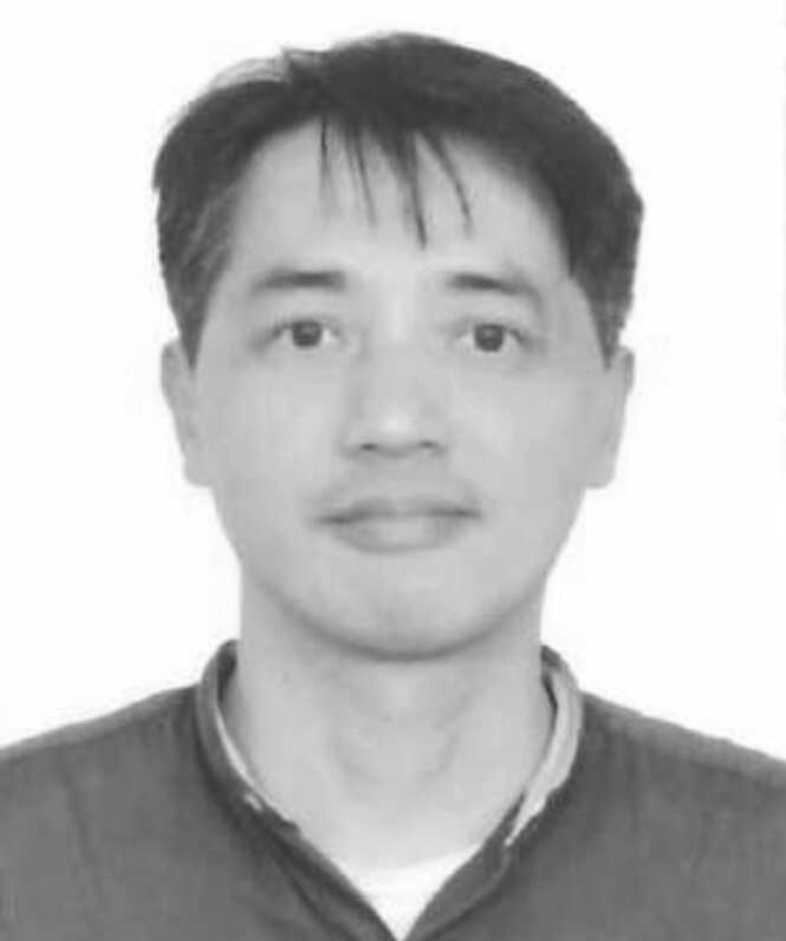
\includegraphics[width=1in,height=1.25in,clip,keepaspectratio]{Figure/author/Peng Un Mak.png}}]
  {Peng Un Mak} (Senior Member, IEEE) (S'88-M'97-SM'11-18, 20) received the B.Sc. degree in electrical engineering from National Taiwan University, Taipei, Taiwan in 1986, and the M.Sc. and Ph.D.\ degrees in electrical engineering from Michigan State University, East Lansing, MI, USA in 1990 and 1997 respectively.
  Since 1997, he has been an Assistant Professor with the Department of Electrical and Computer Engineering, Faculty of Science and Technology, University of Macau, Macau SAR, China.
  His current research interests include biosignal extraction and processing, bioelectromagnetism, human body communication, and body sensor networks.
  He was a visiting scholar at Department of Physiology and Biophysics, School of Medicine, the Anschutz Medical Campus, University of Colorado, Denver, CO, USA, in 2012/2013.
  Also he was a Visiting Fellow at Clare Hall in the University of Cambridge, Cambridge, U.K., in 2018.
  He is a currently a Life Member of both the Phi Kappa Phi and Clare Hall.
  In addition, he is an Invited Member of the Eta Kappa Nu (currently IEEE-HKN).
\end{IEEEbiography}




\begin{IEEEbiography}[{
\includegraphics[width=1in,height=1.25in,clip,keepaspectratio]{Figure/author/Mang I Vai.png}}]
{Mang I Vai} (Senior Member, IEEE)  received the Ph.D. degree in electrical and electronics engineering from the University of Macau, SAR, China, in 2002. Since 1984, he has been performing research in the areas of digital signal processing and embedded systems. He is now the coordinator of the State Key Laboratory of Analog and Mixed-Signal VLSI and an associate professor of Electrical and Computer Engineering, Faculty of Science and Technology, University of Macau.
\end{IEEEbiography}




\end{document}